%\chapter{Architektur}
\chapter{\colorbox{yellow}{Architektur}}

%Graph mit allen Tools, Architektur in Graph zeigen
%Beschreibung alles Frameworks, die in Prototyp verwendet werden
%DI in Backend und DI in Frontend, reference auf Kapitel Theorie->DI

Der webbasierte Foto-Verwaltungs-Service wird auf Basis des \textbf{MVC-}Pattern entwickelt, welcher aus drei Komponenten (Model, View und Controller) besteht. Der Backend-Teil enthält das Model. Zwei weitere Komponente, View und Controller befinden sich im Frontend-Teil der Webanwendung. View übernimmt die Verantwortung für die Gestaltung der Webseite und Controller wird in JavaScript implementiert, der die Client-Anfragen entsprechend bearbeitet \textbf{(Abb. \ref{img:architectureMyApp})}.

Der Zugriff auf Funktionen auf der Serverseite erfolgt über \textit{REpresentational State Transfer} oder kurz \textbf{REST}. Durch die Verwendung von REST erfolgen die Web-Client-Anfragen auf Basis des \textbf{HTTP}\footnote{\textbf{HTTP} ist ein zustandloses Protokoll zur Übertragung der Daten zwischen Web-Client (= Browser Anwendung) und Web-Server. Jede neue Anfrage, die vom Web-Client erfolgt, erfordert einen neuen Verbindungsaufbau und erneute Datenbeschaffung.}-Protokolls. Der Web-Client sendet \textbf{HTTP}-Request und erwartet \textbf{HTTP}-Response, in dem Fall des implementierten Prototyps im \textit{JSON}\footnote{JSON (JavaScript Object Notation), \url{http://www.json.org}}-Format.

Die Skalierung der Daten findet auf der Datenbankebene statt. Im Fall des implementierten Prototyps übernimmt die Verantwortung für die Skalierbarkeit \mongo, eine dokumentenorientierte \textit{NoSQL}-Datenbank.

\colorbox{red}{Die rechtzeitige Synchronisation von Daten wird nicht in Kauf genommen.}

Der Zustand \textit{(= Session)} der Web-Client-Anfragen wird im Frontend-Teil implementiert. Der Web-Server enthält keine Information über Session, da dieser \textit{stateless} arbeitet. \textit{Stateless} bedeutet, dass die Web-Clients mit jeder Anfrage einen neuen Verbindungsaufbau und erneute Datenbeschaffung erfordern und diese voneinander unabhängig sind. Gleich nach einer Web-Server Response wird die Verbindung geschlossen und der Zustand bleibt nicht gespeichert. Somit ist bei einer \textit{stateless-}Webanwendung Sessions nicht möglich.

Falls nach dem Anwendungskontext eine Zustandsspeicherung gefordert wird, wäre die Umsetzung in einer \textit{stateful}-Webanwendung möglich. Bei einer \textit{stateful}-Webanwendung werden Web-Client Anfragen zu einer gemeinsamen logischen Sitzung zusammengefasst, um alle Nutzerinteraktionen hinweg in einem einzigen Kontext auszuführen. Dies wird mithilfe von \textit{Session-Cookies}\footnote{Session-Cookie, \url{https://help.sap.com/erp2005_ehp_04/helpdata/de/cc/d6eef928f711d5991f00508b6b8b11/content.htm}, zugegriffen am 20.01.2017} realisiert.

\begin{figure}[H]
\centering
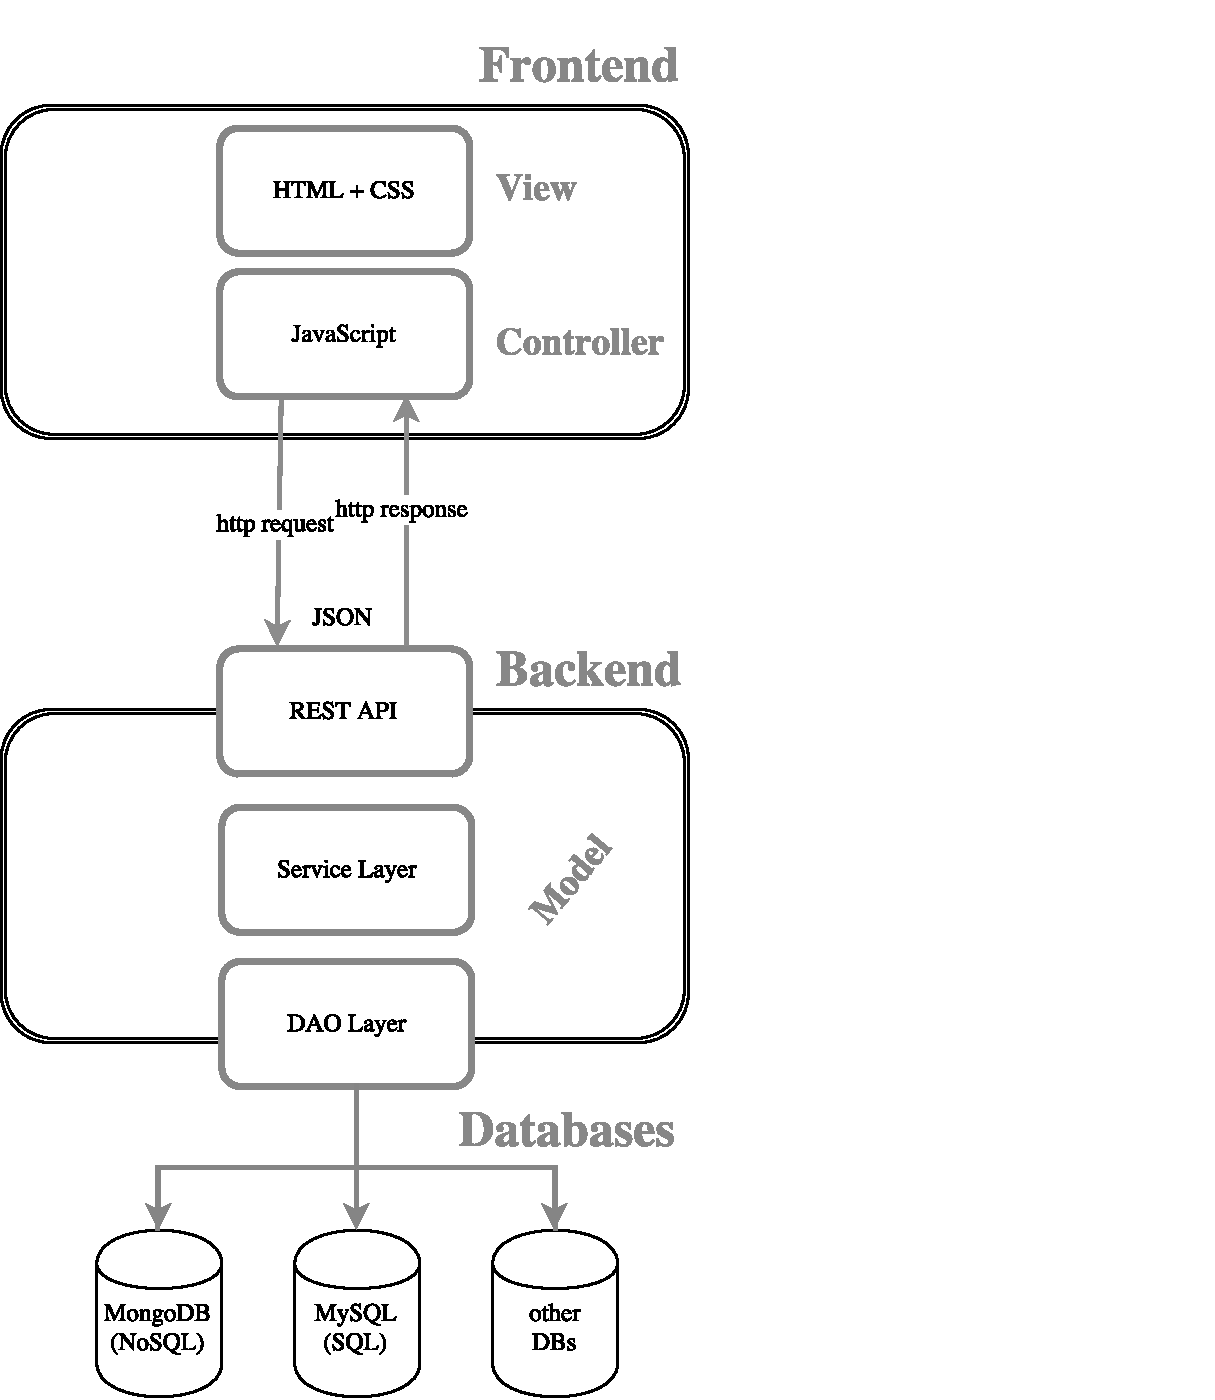
\includegraphics[trim = 0mm 0mm 0mm 0mm, clip, width=0.4\textwidth]{resources/architectureMyAppWithoutFrameworks}
\caption[Architektur-Prototyp]{Architektur-Prototyp}
\label{img:architectureMyApp}
\end{figure}

%\begin{wrapfigure}{r}{0.4\textwidth}
%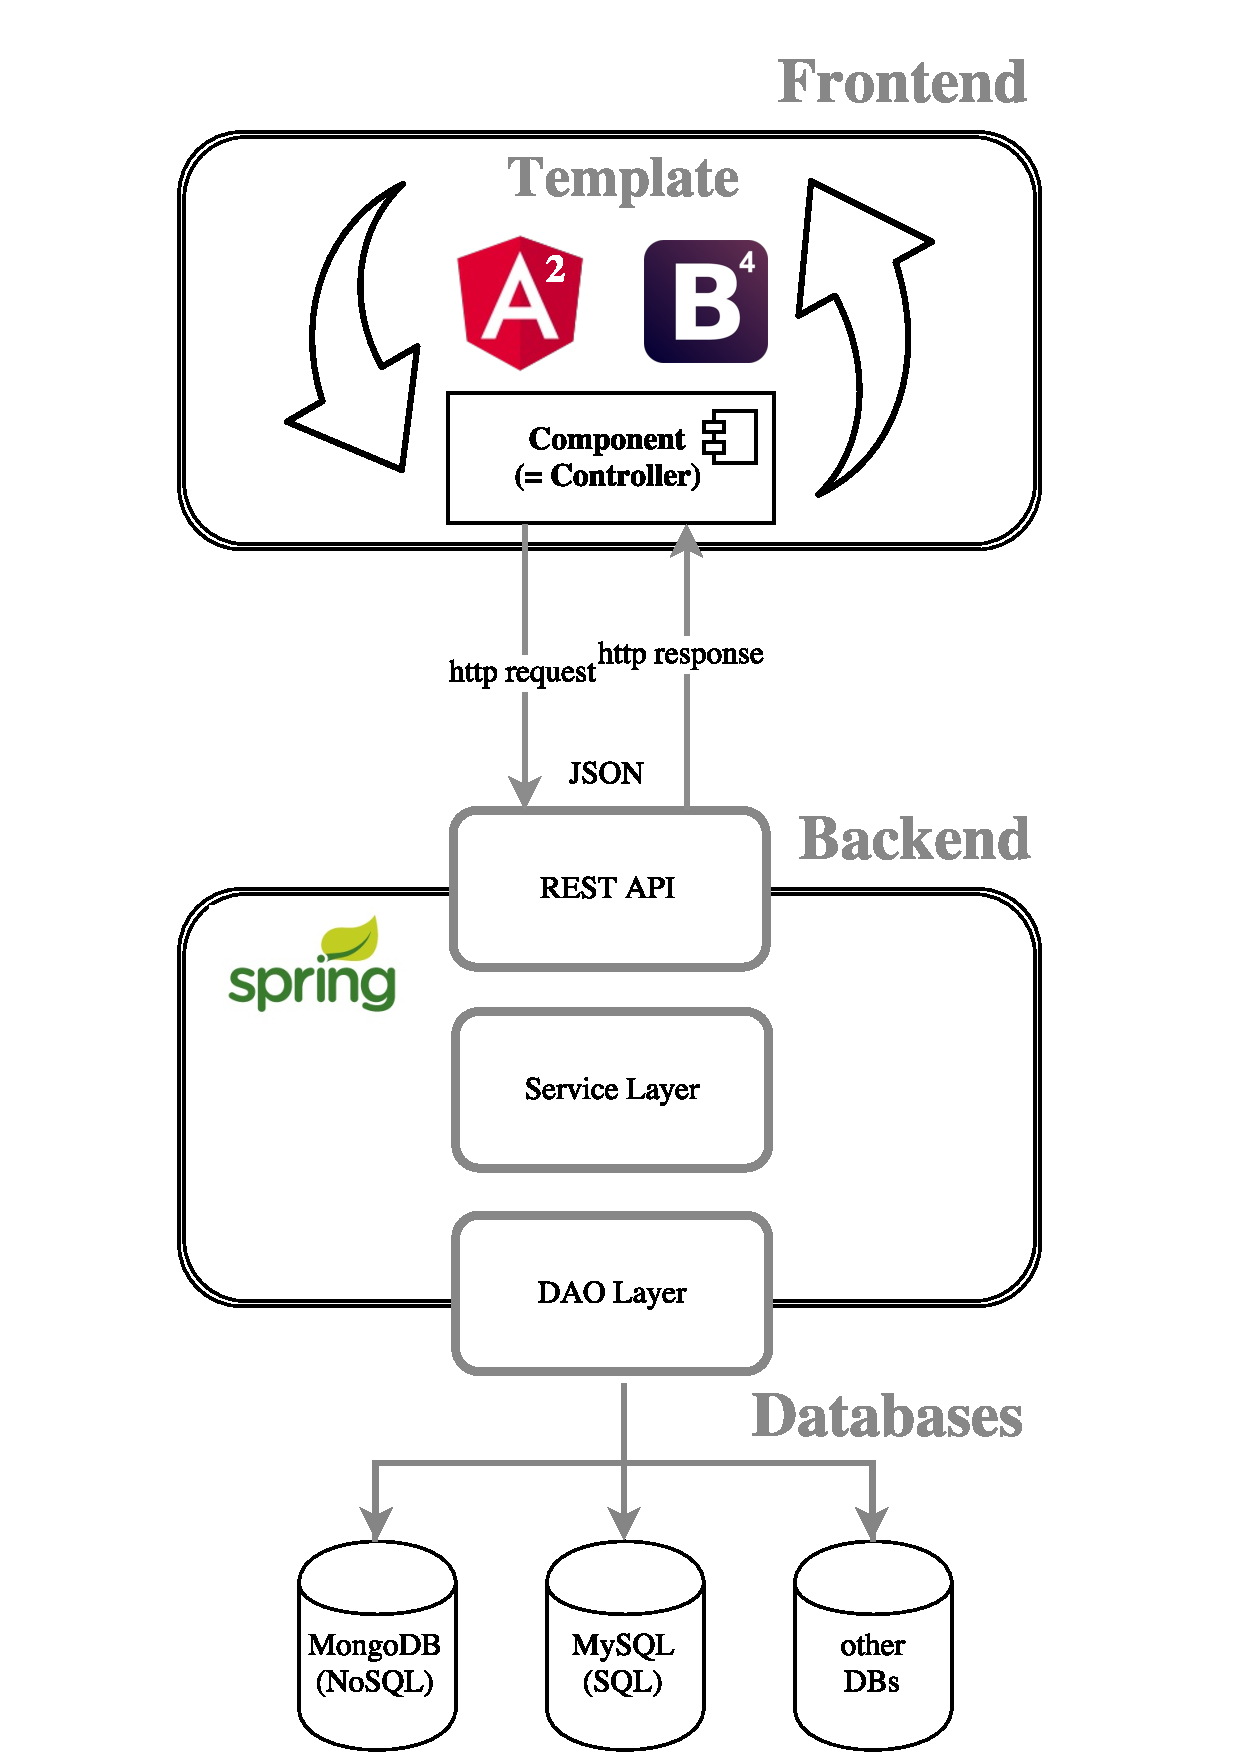
\includegraphics[trim = 20mm 0mm 30mm 9mm, clip, width=0.4\textwidth]{resources/architectureMyApp}
%\caption[Architektur-Prototyp]{\label{img:myArchitecture}Architektur-Prototyp}
%\end{wrapfigure}

%\section{Datenhaltungsschicht (Databases)}
\section{\colorbox{yellow}{Datenhaltungsschicht (Databases)}}

Im Vergleich zu den relationalen Datenbanken, die sich als eine strukturierte Sammlung von Tabellen (den Relationen) vorstellen, in welchen Datensätze abgespeichert sind, eignen sich \textit{NoSQL}-Datenbanken zur unstrukturierter Daten, die einen nicht-relationalen Ansatz verfolgen. 

%\subsection{NoSQL-Datenbanken}
\subsection{\colorbox{yellow}{NoSQL-Datenbanken}}

Der Begriff NoSQL steht nicht für 'kein SQL', sondern für 'nicht nur SQL' (Not only SQL). Das Ziel von NoSQL ist, relationale Datenbanken sinnvoll zu ergänzen, wo sie Defizite aufzeigen. Entstanden ist dieses Konzept in erster Linie als Antwort zur Unflexibilität, sowie zur relativ schwierigen Skalierbarkeit von klassischen Datenbanksystemen, bei denen die Daten nach einem stark strukturierten Modell gespeichert werden müssen.\footnote{MySQL vs. MongoDB: \url{http://www.computerwoche.de/a/datenbanksysteme-fuer-web-anwendungen-im-vergleich,2496589}, zugegriffen am 3. Januar 2016} Dokumentdatenbanken gruppieren die Daten in einem strukturierten Dokument, typischerweise in einer \textit{JSON}-Datenstruktur. \mongo\ ist eine von vielen NoSQL-Datenbanken, die auch diesen Ansatz verfolgt und bietet darauf aufbauend eine reichhaltige Abfragesprache und \textit{Indexe} auf einzelne Datenfelder. Die Möglichkeiten der \textit{Replikation} und des \textit{Shardings} zur stufenlosen und unkomplizierten Skalierung der Daten und Zugriffe macht \mongo\ auch für stark frequentierte Websites äußerst interessant.(\cite{Hollosi.2012}, Kapitel 14, Seite 435)

Beispiele für NoSQL-Datenbanken:
\begin{multicols}{2}
\begin{itemize}
\item CouchDB
\item MongoDB
\item Redis
\item Google BigTable
\item Amazon Dynamo
\item Apache Cassandra
\item Hbase (ApacheHadoop)
\item Twitter Gizzard
\item weitere…
\end{itemize}
\end{multicols}

Jede NoSQL-Datenbank verfolgt seine eigene Ziele.

%\subsubsection{Kategorien von NoSQL-Systemen}
\subsubsection{\colorbox{yellow}{Kategorien von NoSQL-Systemen}}

\begin{itemize}
\item Eine Key-Value-Datenbank \textit{(Key-Value Store)} ist eine Datenbank, in der die Daten in Form von Schlüssel-Werte-Paaren abgespeichert werden. Der Schlüssel verweist dabei auf einen eindeutigen (meist in Binär- oder Zeichenketten-Format vorliegenden) Wert\footnote{NoSQL: Key-Value-Datenbank Redis im Überblick: \url{https://www.heise.de/developer/artikel/NoSQL-Key-Value-Datenbank-Redis-im-Ueberblick-1233843.html}, zugegriffen am 17. Januar 2017}. Value kann oft beliebiger Datentyp wie Arrays, Dokumente, Objekte, Bytes etc. sein.

\item In einer spaltenorientierten Datenbank \textit{(Column Store)}, wie der Name vermuten lässt, werden die Datensätze spalten- statt zeilenweise abgespeichert. Durch die spaltenorientierte Abspeicherung der Daten wird der Lesezugriff stark beschleunigt, da keine unnötigen Informationen mehr gelesen werden, stattdessen nur diejenigen, die wirklich benötigt wurden. Dadurch wird der Schreibprozess aber erschwert, falls die schreibenden Daten aus mehreren Spalten bestehen werden, auf die entsprechend zugegriffen werden muss. Der Schreibprozess wird sich in diesem Fall etwas verlangsamen.

\item Eine Graphen-Datenbank \textit{(Graph database)} ist die weitere Kategorie aus der NoSQL Gruppe, in der die Daten anhand eines Graphen dargestellt und abgespeichert werden.

Die Graphen bestehen grundsätzlich aus Knoten \textit{(Node)} und Kanten \textit{(Edge)}. Dabei stellen die Kanten die Verbindungen zwischen den einzelnen Knoten dar.

\item Eine Datenbank, in der die Daten in Form von Dokumenten abgespeichert werden, ist als eine dokumentenorientierte Datenbank \textit{(Document Store)} zu definieren. In diesem Zusammenhang ist ein Dokument als eine Zusammenstellung bestimmter Daten zu verstehen, das mit einem eindeutigen Identifikator angesprochen werden kann. Da die Daten in der dokumentenorientierten Datenbank nicht in Form von Tabellen, sondern in Form von Dokumenten abgespeichert werden, ergibt sich daraus keinen Strukturzwang.

Möchte man ein bestimmtes Dokument erweitern, so kann man es einfach tun, da eine dokumentenorientierte Datenbank strukturfrei ist. Weitere Datenformate sind beispielsweise YAML\footnote{YAML: \url{http://www.yaml.org/start.html}} (angelehnt an XML) oder XML\footnote{XML: \url{https://www.xml.com/}} selbst. 
\end{itemize}

Bei dem Auswahl einer Datenbank für Foto-Verwaltungs-Service fiel die Entscheidung auf eine der NoSQL-Datenbank \mongo. Laut DB-Ranking\footnote{DB-Ranking: \url{http://db-engines.com/de/ranking}, zugegriffen am 13. März 2017} ist die \mongo\ einer der populärsten Datenbanken aus der NoSQL-Gruppe und passt ideal für Webprojekte mit \textit{Big Data}.

%\section{MongoDB}\label{mongo}
\section{\colorbox{yellow}{MongoDB}}\label{mongo}

\mongo\ ist eine  schemalose, dokumentenorientierte Open-Source-Datenbank. Der Name stammt von dem englischen Begriff \textit{hu}MONGO\textit{us}, ins Deutsche als \textit{gigantisch} oder \textit{riesig} übersetzen lässt. Die genannte NoSQL-Datenbank macht mit seinem effizienten dokumentenorientierten Ansatz, einfacher Skalierbarkeit und hoher Flexibilität dem bewährten MySQL\footnote{MySQL: \url{https://www.mysql.com}}-System zunehmend Konkurrenz.\footnote{MySQL vs. MongoDB: \url{http://www.computerwoche.de/a/datenbanksysteme-fuer-web-anwendungen-im-vergleich,2496589}, zugegriffen am 19. Januar 2017} 


\rowcolors{1}{white}{lightgray}
\newcommand*{\head}[1]{\textbf{#1}}%

\rowcolors{2}{gray!25}{white}
\begin{table}[h]
\centering
\begin{tabular}{cc}
\toprule 
    \rowcolor{gray!50}
	Relational & \mongo\ \\
	\midrule
	Database &  Database\\
	Table & Collection\\
	Row &  Document\\
	Column &  Field\\
	Index & Index\\
	Join &  Embedding and Linking\\
	Primary key & \textit{\_id}-Field (default)\\
	\bottomrule
\end{tabular}
\caption[Konzepte im Vergleich]{Konzepte im Vergleich}
\label{table:concepts}
\end{table}

\mongo\ präsentiert sich als eine quelloffene, dokumentenorientierte NoSQL-Datenbank mit den folgenden Konzepten wie \textit{Ausfallsicherheit} und \textit{horizontale Skalierung}, deren Bedeutung im Einzelnen in folgenden Unterkapiteln zu erläutern sind.
Die Unterschiede zu den Konzepten der relationalen und nicht-relationalen Datenbanken konkret von \mongo\ stellt die Tabelle \ref{table:concepts} dar.

\subsection{\colorbox{yellow}{Datensätze in Form von Dokumenten}}
%\subsection{Datensätze in Form von Dokumenten}
Die Datensätze werden in  der NoSQL-Datenbank \mongo\ in Dokumente gespeichert. \mongo\ verwendet für die Dokumentenspeicherung und den Datenaustausch das sogenannte \textbf{BSON}\footnote{BSON: \url{http://www.bjson.org}}-Format, das eine binäre Darstellung von \textbf{JSON}-ähnlichen Dokumenten bietet. Nachfolgend sind alle für \textbf{BSON} definierten Datentypen aufgelistet:
\begin{multicols}{3}
\begin{itemize}
\item Double
\item String
\item Object
\item Array
\item Binary Data
\item Undefined
\item Object Id
\item Boolean
\item Date
\item Null
\item Regular Expression
\item JavaScript
\item Symbol
\item JavaScript(with scope)
\item 32-Bit Integer
\item Timestamp
\item 64-Bit Integer
\item Min Key
\item Max Key
\end{itemize}
\end{multicols}
Der Grund für die große Anzahl an Datentypen ist ein wesentliches Ziel der Entwickler von \textbf{BSON}: \textit{Effizienz.}

%speichert Daten in Form von Dokumenten im \textbf{BJSON}\footnote{BSON: \url{http://www.bjson.org}}-Format.
Die Dokumente selbst werden von \mongo\ in sogenannten Kollektionen \textit{(Collections)} gespeichert, die grob mit den Tabellen einer relationalen Datenbank vergleichbar sind. Ein Zugriff auf Daten mehrerer Kollektionen \textit{(Collections)} ist nicht möglich, wie es aus dem \textit{Joins}-Konzept relationaler Datenbank bekannt ist. Die \textit{CRUD}-Operationen sind auf Ebene der \textit{Collection} durchzuführen. Jedes Dokument ist an keine vordefinierte Struktur gebunden und kann eine beliebige Anzahl an Feldern besitzen. Die Dokumente aus einer \textit{Collection} sind komplett unabhängig voneinander. 

Zudem dürfen Dokumente auch innerhalb eines Dokuments gespeichert werden\footnote{Einführung in MongoDB: \url{https://www.iks-gmbh.com/assets/downloads/Einfuehrung-in-MongoDB-iks.pdf}, zugegriffen am 19. Januar 2017}. 

Die Speicherung von Daten in Form von Dokumenten bietet den Vorteil, das sowohl strukturierte, als auch semi-strukturierte und polymorphe Daten gespeichert werden können. Dokumente, die jedoch das gleiche oder ein ähnliches Format haben, sollten zu einer Kollektion \textit{(Collection)} zusammengefasst werden\footnote{MongoDB: \url{http://www.moretechnology.de/mongodb-eine-dokumentenorientierte-datenbank/}, zugegriffen am 21. Januar 2017}.

\subsection{\colorbox{yellow}{Die Architektur}}
%\subsection{Die Nexus Architektur}

Zu den wichtigsten Eigenschaften, die für einen Einsatz von \mongo\ sprechen, gehören:
\begin{itemize}
\item Verfügbarkeit: Auch bei Ausfall einer Datenbankinstanz soll die Anwendung weiterhin verfügbar bleiben.
\item Skalierbarkeit: Mit \textit{Sharding}, einem Verfahren zur horizontalen Skalierung, kann der effiziente Umgang mit großen Datenmengen erreicht werden.\footnote{MongoDB Eigenschaften: \url{https://entwickler.de/online/datenbanken/mongodb-erfolgreich-ein-dokumentenorientiertes-datenbanksystem-einfuehren-115079.html}, zugegriffen am 12. Dezember 2016}
\end{itemize}

%Die Vorteile relationaler und NoSQL-Datenbanken sind aus der Abbildung \ref{img:architektur} zu entnehmen.
%\begin{figure}[H]
%\centering
%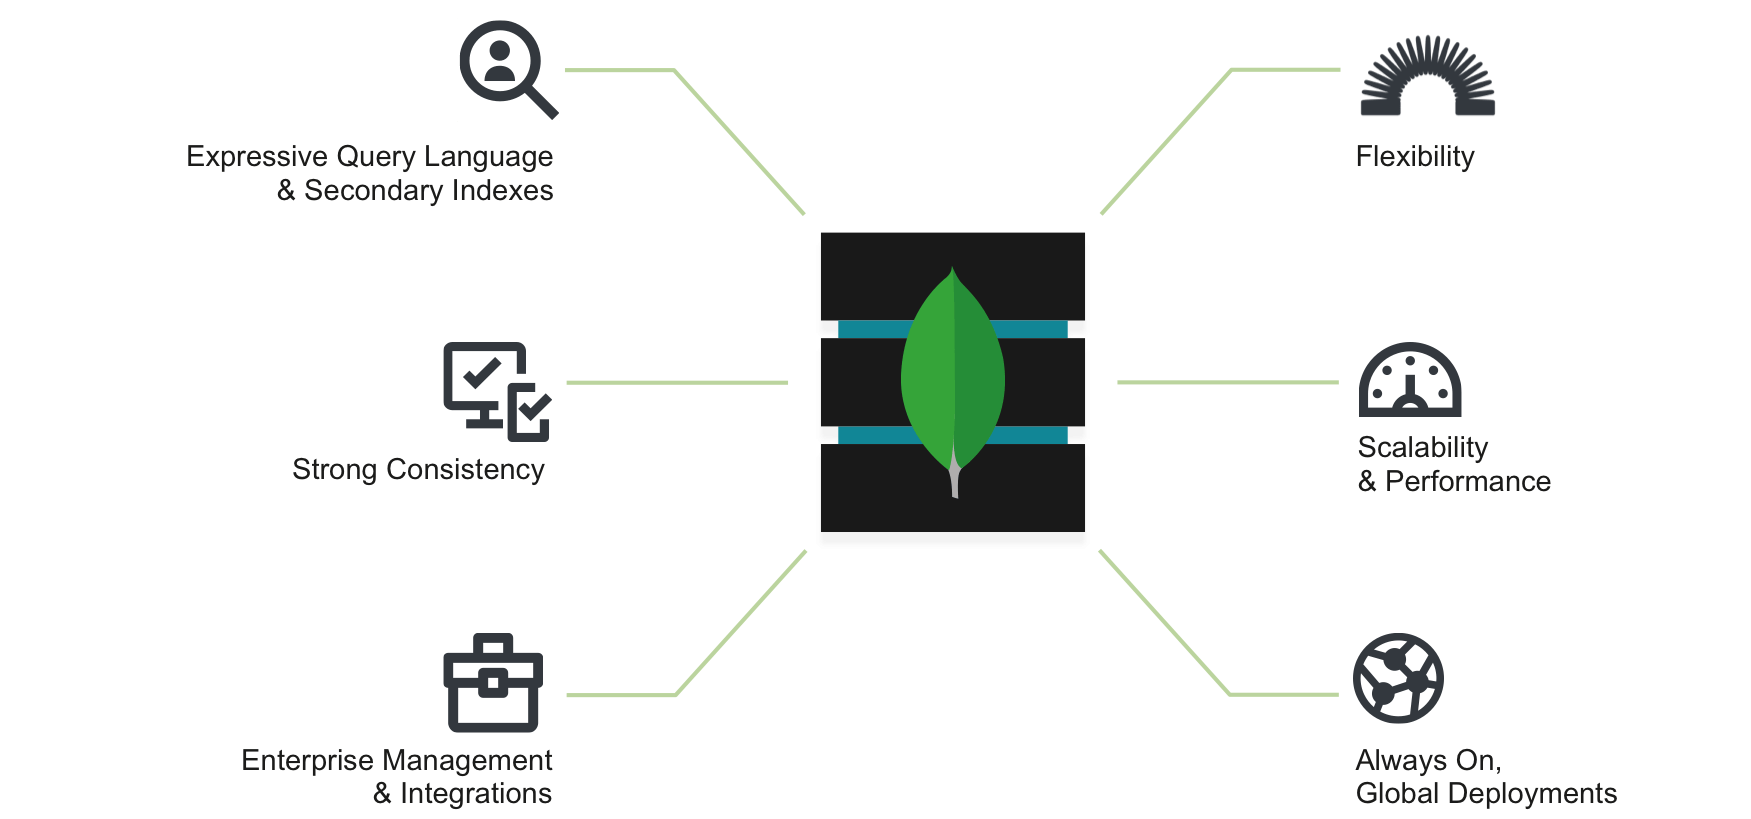
\includegraphics[width=1.0\textwidth]{resources/architecture}
%\caption[MongoDB Architektur]{MongoDB Architektur\protect\footnotemark}
%\label{img:architektur}
%\end{figure}
%\footnotetext{MongoDB Architektur: \url{https://www.mongodb.com/mongodb-architecture}, zugegriffen am 28. Januar 2016}

\subsection{\colorbox{green}{Server/Client starten}}
%\subsection{Server/Client starten}
Zum Starten des Server-Prozesses muss im Terminal der folgende Befehl ausgeführt werden:
\begin{listingsboxShell}[label={lst:serverStart}]{myshell}{Server-Prozess starten}
vlfa:~ vlfa$ mongod
\end{listingsboxShell}
Mit dem Befehl (\textbf{List. \ref{lst:mongoClient}})
\begin{listingsboxShell}[label={lst:mongoClient}]{myshell}{Client-Prozess starten}
vlfa:~ vlfa$ mongo
\end{listingsboxShell}
wird ein Client-Prozess gestartet, falls die \textit{mongod-}Instanz aktiv ist.
Nachdem das Client-Prozess gestartet ist, kann der Client an der Datenbank berühmte \textit{CRUD-}Operationen (\textbf{Kap. \ref{ifur}}) ausführen.

Ohne irgendeine Konfiguration vornehmen zu müssen, verwendet \mongo-Server von Anfang an als Default den TCP-IP-Port 27017 für eingehende Verbindungen.

\mongo\ unterstützt auch eine HTML-basierte Administrationsoberfläche. Falls sie benötigt wird, ist es möglich, im Terminal mit dem folgenden Befehl die HTML-basierte Administrationsoberfläche zu starten:
\begin{listingsboxShell}[label={lst:html}]{myshell}{HTML-basierte Administrationsoberfläche starten}
vlfa:~ vlfa$ mongod --httpinterface --rest
\end{listingsboxShell}
und dementsprechend sie im beliebigen Browser der folgenden URL aufzurufen:
\begin{listingsboxShell}[label={lst:browser}]{myshell}{HTML-basierte Administrationsoberfläche aufrufen}
http://localhost:28017/
\end{listingsboxShell}
Auf der Seite sind alle relevante Informationen zu Replikaktionsgruppen, Skalierung, verbundene Clients etc. zu finden.


\subsection{\colorbox{green}{CRUD = IFUR-Operationen}\label{ifur}}
%\subsection{CRUD = IFUR-Operationen}\label{ifur}
Die \textit{\textbf{CRUD}}-Operationen aus SQL heißen in \mongo\ \textit{\textbf{I}nsert}, \textit{\textbf{Fi}nd}, \textit{\textbf{U}pdate} und \textit{\textbf{R}emove}. Bei \mongo\ ist es nicht einmal notwendig, eine Datenbank oder eine Collection zu definieren, bevor etwas gespeichert wird. Datenbanken und Collections werden zur Laufzeit beim ersten Einfügen eines Dokuments von MongoDB erzeugt.
\subsubsection{Create/Insert}
Für die Speicherung von neuen Dokumenten in der Datenbank bietet \mongo\ drei Funktionen (\textbf{Listing \ref{lst:insert}}) an, welche als Parameter ein einzelnes oder eine Reihe von Dokumenten in einem Array annehmen. %Die \textit{Collection} muss vor dem Einfügen von neuen Dokumenten nicht explizit angelegt werden. Falls sie nicht existiert, wird sie zunächst erstellt und die übergebenen Dokumente eingefügt.
\begin{listingsboxShell}[label={lst:insert}]{myshell}{Dokument(e) speichern}
> db.<collection>.insert(<...>)
> db.<collection>.insertMany(<...>)
> db.<collection>.insertOne(<...>)
\end{listingsboxShell}
\mongo\ generiert für jedes neues Dokument eine ID mit dem Feldnamen \textit{\_id}, falls keine konkrete Dokument\_ID angegeben ist.

\subsubsection{Read/Find}
Zum Durchsuchen nach Dokumenten mit bestimmten Eigenschaften bietet \mongo\ drei weitere Funktionen (\textbf{Listing \ref{lst:find}}) an. Das Ergebnis beim Aufruf einer der folgenden Funktionen ist ein Cursor, der auf alle passenden Dokumente zeigt.
\begin{listingsboxShell}[label={lst:find}]{myshell}{Dokument(e) finden}
> db.<collection>.find(<...>)
> db.<collection>.findOne(<...>)
> db.<collection>.findOneAndDelete(<...>)
\end{listingsboxShell}
\subsubsection{Update/Update}
Die drei nächsten Funktionen (\textbf{Listing \ref{lst:update}}) ermöglichen, anhand des Inhalts bestimmte Dokumente zu filtern und in diesen Änderungen durchzuführen. Die Änderungen umfassen das Hinzufügen, Entfernen oder Umbenennen von Feldern.
\begin{listingsboxShell}[label={lst:update}]{myshell}{Dokument(e) aktualisieren}
> db.<collection>.update(<...>)
> db.<collection>.updateMany(<...>)
> db.<collection>.updateOne(<...>)
\end{listingsboxShell}
\subsubsection{Delete/Remove}
Das Löschen von ganzen Dokumenten erfolgt in \mongo\ anhand der folgenden Funktion (\textbf{Listing \ref{lst:remove}}), indem beim Aufruf entsprechende Informationen für die Dokumente angegeben werden.
\begin{listingsboxShell}[label={lst:remove}]{myshell}{Dokument(e) löschen}
> db.<collection>.remove(<...>)
\end{listingsboxShell}

\subsection{\colorbox{green}{Indizes}}
%\subsection{Indizes}
Um die Laufzeit von Datenbankabfragen zu optimieren bzw. zu beschleunigen, können Indexe verwendet werden. Indexe in MongoDB werden als \textit{B-Tree}-Datenstrukturen\footnote{B-Tree-Datenstrukturen: \url{https://de.wikipedia.org/wiki/B-Baum}, zugegriffen am 10. Februar 2017} verwaltet.

Neben dem obligatorischen Primär-Index auf dem Feld \textit{\_id} ist es möglich, beliebige Sekundärindexe anzulegen. Insgesamt erlaubt \mongo\, pro Collection auf einzelnen Feldern oder einer Gruppe von Feldern bis zu 64 Indexe zu definieren.

Auf der Kommandozeile ist es möglich, das Administrationswerkzeug \textit{Mongo Shell} zu verwenden, um mit einer Collection aus einer Datenbank verbinden zu können. Indexe anzulegen, ermöglicht \mongo\ mit dem folgenden Befehl (\textbf{Listing \ref{lst:createIndex}}). 
\begin{listingsboxShell}[label={lst:createIndex}]{myshell}{Index auf ein Feld anlegen}
> db.<collection>.createIndex( {<feld>: 1} )
\end{listingsboxShell}
%\subsubsection{Creating Indexes}
%blabla
%
%\begin{listingsboxShell}[label={lst:X}]{myshell}{Mongo-Shell: Something else}
%> db.students.createIndex();
%\end{listingsboxShell}
%
%blabla
%
%\begin{listingsboxShell}[label={lst:X}]{myshell}{Mongo-Shell: Something else}
%> db.students.explain().find();
%\end{listingsboxShell}
%
%Quiz: Please provide the mongo shell command to add an index to a collection named students, having the index key be class, student\_name.
%Neither will go in the "-1" direction..
%
%\begin{listingsboxShell}[label={lst:X}]{myshell}{Something else}
%> db.students.createIndex({student\_name:1, class:1});
%\end{listingsboxShell}
%
%\begin{listingsboxShell}[label={lst:X}]{myshell}{Mongo-Shell: Something else}
%> db.students.dropIndex({student_name:1});
%\end{listingsboxShell}
%
%\subsubsection{Multikey Indexes}
%blabla
%\subsubsection{Index Creation Option, Unique}
%für jedes attribut kann man Unique definieren, d.h. doppelte Werte dürfen nicht vorkommen\newline\newline
%
%\begin{listingsboxShell}[label={lst:X}]{myshell}{Mongo-Shell: Something else}
%> db.students.createIndex({student_id : test}, {unique:true});
%\end{listingsboxShell}
%
%Please provide the mongo shell command to create a unique index on student\_id, class\_id, ascending for the collection students.
%
%\begin{listingsboxShell}[label={lst:X}]{myshell}{Mongo-Shell: Something else}
%> db.students.createIndex({student_id:1, class_id:1}, {unique:true});
%\end{listingsboxShell}
%
%\subsubsection{Index Creation, Sparse}
%
%Im Fall, wenn ein Attribut nicht in allen Dokumenten vorkommt, aber für dieses ein Unique Index definiert werden soll, muss Folgendes verwendet werden:
%
%\begin{listingsboxShell}[label={lst:X}]{myshell}{Something else}
%> db.students.createIndex({cell:1}, {unique:true, sparse:true});
%\end{listingsboxShell}
%
%blabla, siehe den Shellbefehl, blabla
%
%\begin{listingsboxShell}[label={lst:X}]{myshell}{Something else}
%> db.students.createIndex({student_id:1, class_id:1}, {unique:true});
%\end{listingsboxShell}
%siehe Codeauszug

\subsection{\colorbox{green}{Aggregation}}\label{aggr}
%\subsection{Aggregation}\label{aggr}
\mongo\ bietet eine Menge von Aggregationsoperationen an, die die Datensätze wunschmäßig verarbeiten und die berechneten Ergebnisse zurückliefern. Die Aggregationsoperationen gruppieren Werte aus mehreren Dokumenten zusammen. Des Weiteren ist es möglich, eine Vielzahl von Operationen auf den gruppierten Daten auszuführen, um ein einziges Ergebnis zurückzuliefern. \mongo\ bietet drei Möglichkeiten, Datenaggregation durchzuführen. Diese sind 
\begin{itemize}
\item Aggregation Framework
\item Map/Reduce und
\item Single purpose aggregation.\footnote{Aggregation: \url{https://docs.mongodb.com/manual/aggregation/}, zugegriffen am 1. März 2017}
\end{itemize}
In dieser Arbeit wird auf nur eine der drei Möglichkeiten eingegangen und nicht nur allgemein. Das ist Aggregation Framework. Durch den Ansatz an dem Prototyp (\textbf{Kap. \ref{prototyp}}) wird das Aggregation Framework näher kennengelernt.

\subsubsection{Aggregation Framework}\label{aggrFr}
%Aggregation Framework ist ein Konzept, das \mongo\ für die Datenaggregation modelliert hat, um Entwicklern die Arbeit bei den komplexen Abfragen ohne fundierte JavaScript-Kenntnisse erleichtern zu können. 
Analog zu \textit{GROUP BY} in SQL hat \mongo\ sein eigenes Konzept entwickelt, das im eigenen Aggregation Framework modelliert ist. Welche Möglichkeiten bietet \mongo's Aggregation Framework an, wird im Kapitel \ref{prototyp} mit Anwendungsfällen detailliert erläutert. Die einzelnen Aggregationsoperationen mit entsprechender Beschreibung sind aus der Tabelle \ref{table:aggrOperators} zu entnehmen. Die Datenaggregation durch das Aggregation Framework ist natürlich nicht nur auf \textit{Shell-}Ebene, sondern auch in vielen gängigen Programmiersprachen, wie zum Beispiel Java, C++, C\#, PHP, Python etc. durch bereitgestellte \mongo's Treiber\footnote{MongoDB Drivers: \url{https://docs.mongodb.com/ecosystem/drivers/}, zugegriffen am 18. Januar 2017} möglich.
\begin{table}[H]
\centering
\begin{tabular}{lp{2.3cm}p{10.3cm}}
\toprule 
    \rowcolor{gray!50}
	\mongo & SQL & Beschreibung\\
	\midrule
	\$match & WHERE, HAVING & Der \textit{\$match-}Operator funktioniert nach dem gleichen Prinzip wie \textit{db.<collection>.find({})}.\\
	\$group & GROUP BY & Der \textit{\$group-}Operator gruppiert berechnete Ergebnisse nach bestimmten Feldern.\\
	\$skip & - & Der \textit{\$skip-}Operator ermöglicht, eine bestimmte Anzahl an Dokumenten zu überspringen.\\
	\$limit & - & Der \textit{\$limit-}Operator formuliert eine konkrete Anzahl an zurücklieferenden Dokumenten.\\
	\$sort & ORDER BY & Der \textit{\$sort-}Operator sortiert Dokumente.\\
	\$project  & SELECT & Der \textit{\$project-}Operator ermöglicht, die Form der berechnenden Ergebnisse zu manipulieren, bzw. das zurücklieferende Ergebnis wunschmäßig zu formen-\\
	\$unwind  & - & Der \textit{\$unwind-}Operator dekonstruiert ein Array-Feld aus einem Dokument, falls so ein Array-Feld existiert-\\
	\bottomrule
\end{tabular}
\caption[Aggregationsoperationen]{Aggregationsoperationen}
\label{table:aggrOperators}
\end{table}
%\subsection{Map/Reduce}\label{map}
%\mongo\ bietet auch eine eigene Implementierung des Map/Reduce-Algorithmus an.

\subsection{\colorbox{green}{Horizontale Skalierung (Sharding)}}\label{sharding}
%\subsection{Horizontale Skalierung (Sharding)}\label{sharding}
Um eine kostengünstige Lösung für eine Steigerung der Leistung von Systemen zu ermöglichen, ermöglicht das Datenbanksystem von \mongo\  eine horizontale Skalierung, die allgemein im Teilabschnitt \ref{scale} schon diskutiert ist. Die horizontale Verteilung der Daten erfolgt bei \mongo\ auf Ebene der \textit{Collections} nach \textit{Sharding-Keys}, siehe Abbildung \ref{img:sharding}. Die \textit{Sharding-Keys} (\textbf{Abs. \ref{sharding-keys}}) dienen dazu, um später Zugriffe auf einzelne Dokumente zu ermöglichen.
\begin{figure}[H]
\centering
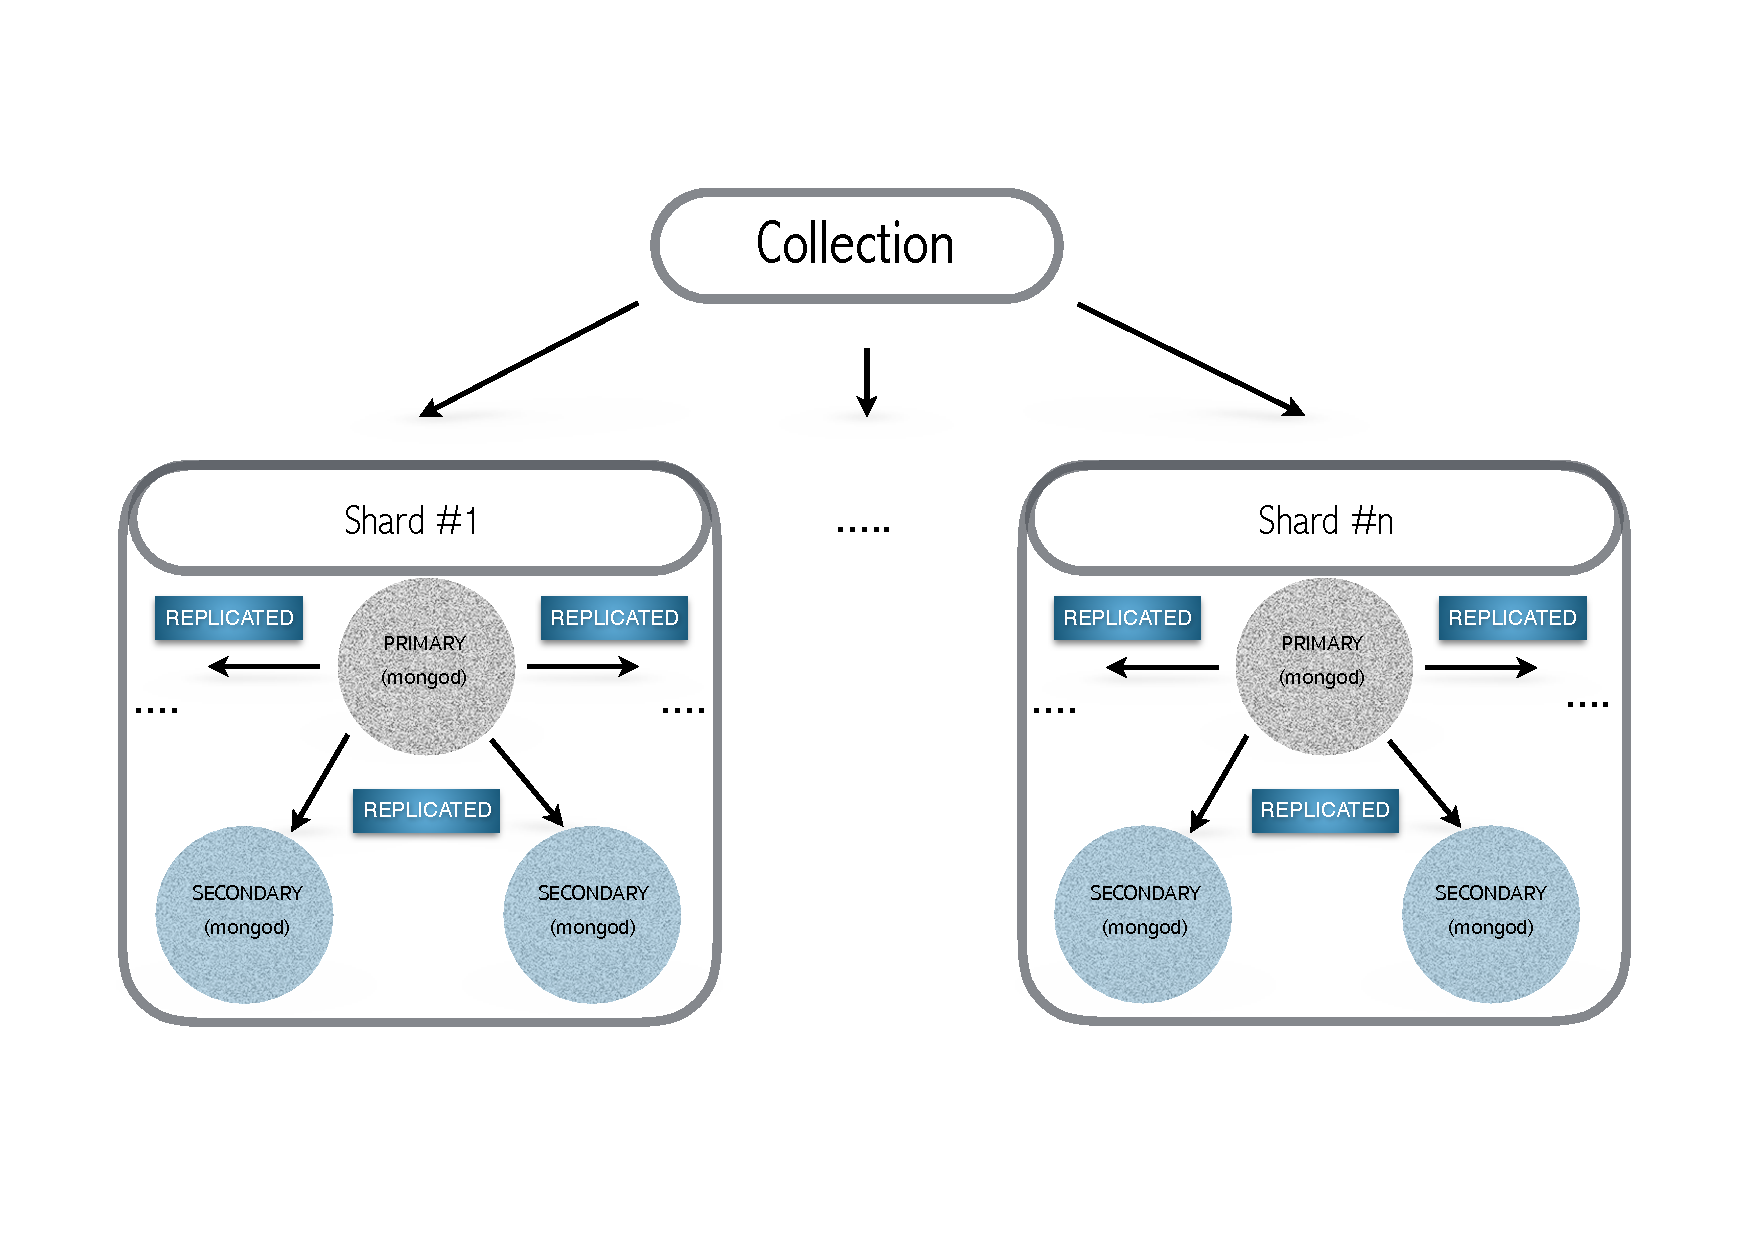
\includegraphics[trim = 0mm 35mm 0mm 30mm, clip, width=1.0\textwidth]{resources/replicaSet/sharding}
\caption[Ein Beispiel für Verteilung einer \textit{Collection} auf mehreren \textit{Shards}]{Ein Beispiel für Verteilung einer \textit{Collection} auf mehreren \textit{Shards}}
\label{img:sharding}
\end{figure}
Die Aufteilung der \textit{Collections} erfolgt in Blocks, auch als \textit{Chunks} genannt. Ein \textit{Chunk} ist ein Teil einer bestimmten \textit{Collection}. Gespeichert werden \textit{Chunks} auf Servern, die in diesem Zusammenhang als \textit{Shards} bezeichnet werden. Was es unter \textit{Shards} zu verstehen ist, erläutert der Teilabschnitt \ref{replication} zur Replikation.

Um die Aufteilung der \textit{Collections} in \textit{Chunks} auf \textit{Shards} realisieren zu können, verwendet \mongo\ folgende Komponenten:
\begin{itemize}
\item \textit{shards:} Die \textit{Shards} enthalten letztendlich die Daten. In einer \textit{Shard} ist es möglich, Replikationsgruppen zu verwenden, näher dazu im Teilabschnitt \ref{replication}.
\item \textit{mongos:} Der \textit{mongos} gilt als ein \textit{RoutingService}, der die Anfragen der Anwendungsschicht entgegennimmt und diese an eine entsprechende \textit{Shard} weiterleitet, die die nötigen Daten enthält.
\item \textit{config servers:} Die Konfigurationsserver speichern die Metadaten für einen Sharded-Cluster. Im Fall einer Schreiboperation entscheiden die Konfigurationsserver, in welchen Chunk auf welchem Shard das entsprechende Dokument eingefügt wird. Bei der Leseoperation geben die Konfigurationsserver den Auskunft darüber, welcher Shard die gewünschten Daten enthält. Bei den Konfigurationsservern handeln es um eine \textit{mongod-}Instanzen.
\end{itemize}
Die folgende Abbildung \ref{img:shardedCluster} veranschaulicht die Interaktion von den gerade genannten Komponenten innerhalb eines Sharded-Cluster:
%\colorbox{red}{graphische Darstellung}
\begin{figure}[H]
\centering
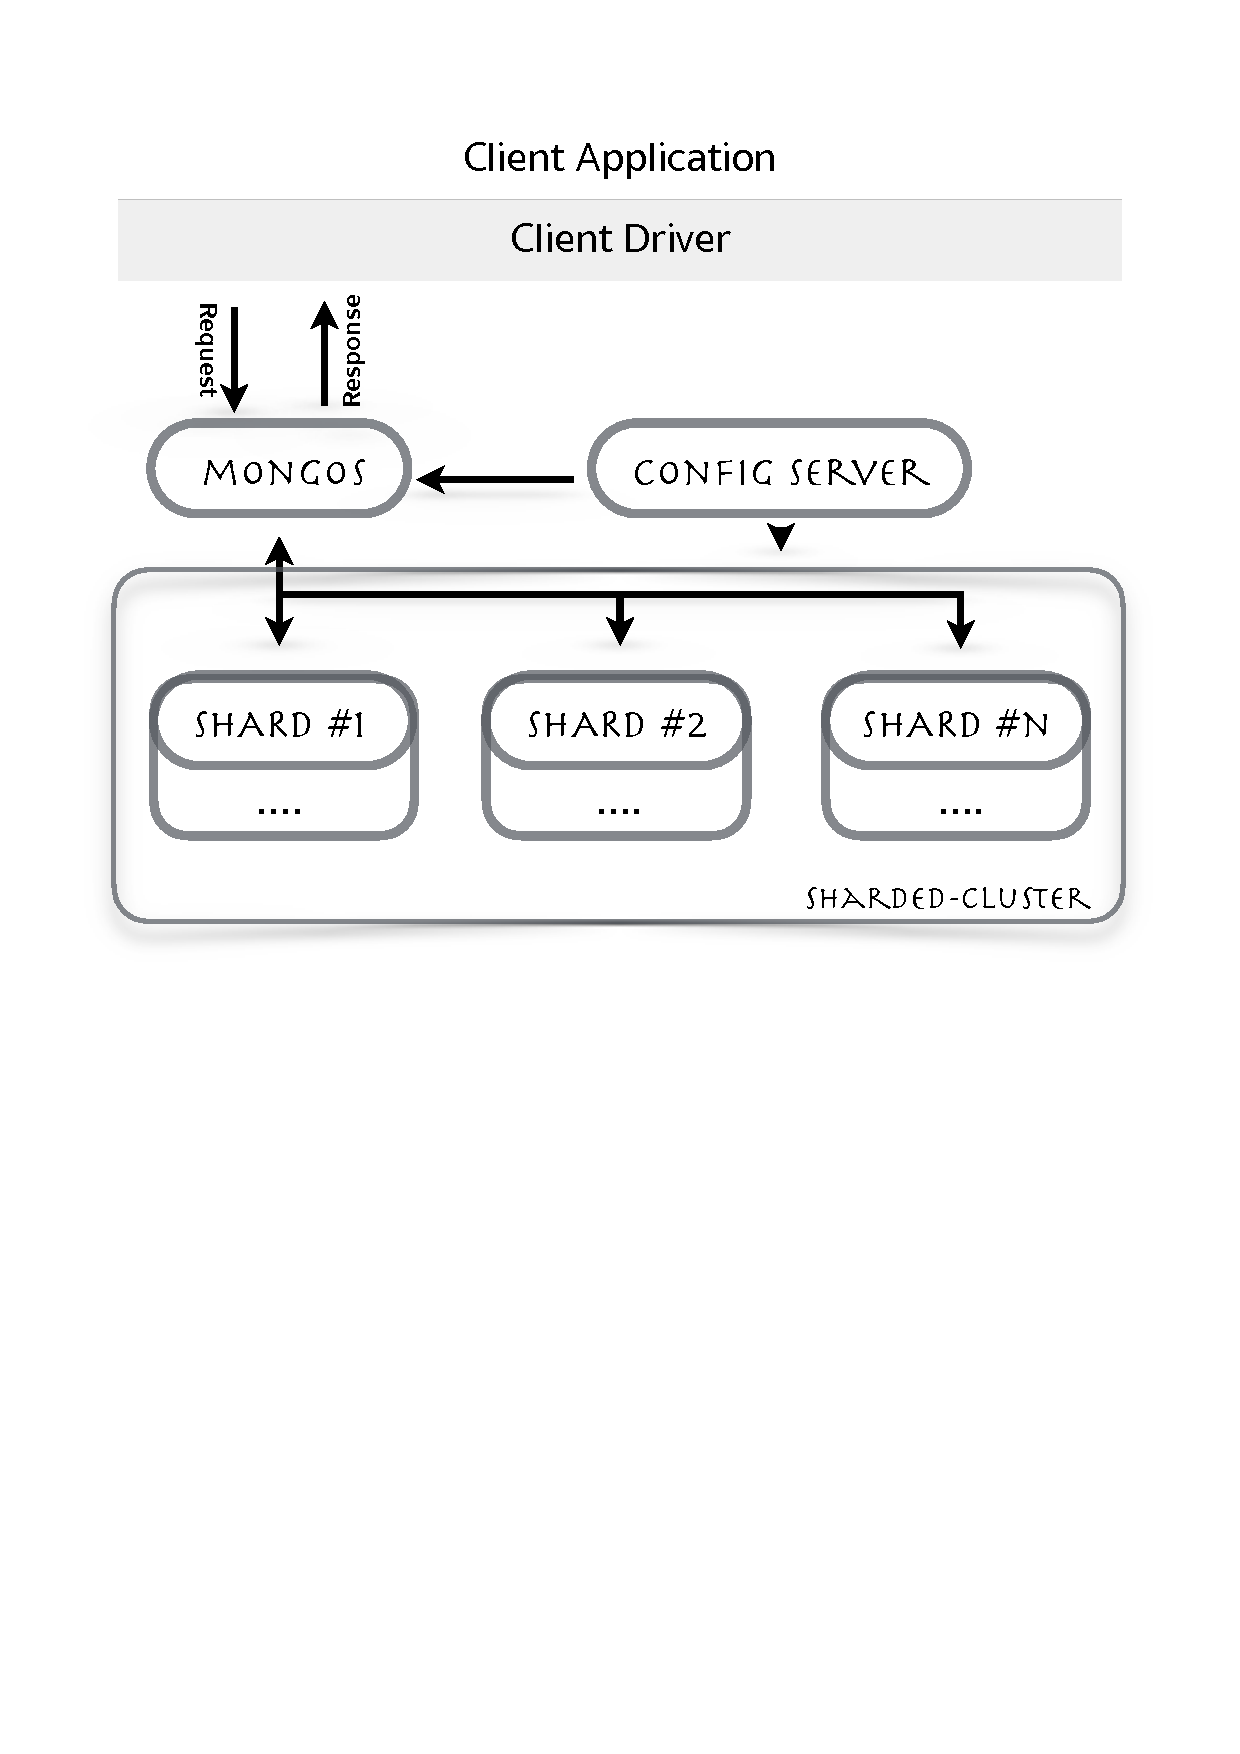
\includegraphics[trim = 0mm 139mm 0mm 22mm, clip, width=0.7\textwidth]{resources/replicaSet/shardedCluster}
\caption[Horizontale Skalierung \textit{(Sharding)}]{Horizontale Skalierung \textit{(Sharding)}}
\label{img:shardedCluster}
\end{figure}

Das Ziel des Ganzen ist die horizontale Skalierbarkeit an Datenmengen, um die Performance des Datenbanksystems zu steigern.

\subsubsection{Fragmentierung des Datenbestands nach \textit{Shard-Keys}}\label{sharding-keys}
Die Fragmentierung des Datenbestands erfolgt auf Ebene der \textit{Collections} nach \textit{Shard-Keys}. In jeder \textit{Collection}  muss ein Schlüssel als sogenannter \textit{Sharding-Key} definiert sein, der entsprechend in jedem Dokument derselben \textit{Collection} existiert.  \textit{Sharding-Key} kann entweder aus einem einzigen indexierten Feld oder einem zusammengesetzten Index bestehen. Die Dokumente werden dann nach \textit{Shard-Key} alphabetisch oder nummerisch sortiert und anschließend in \textit{n-}Blocks gleicher Größe eingeteilt. \mongo\ garantiert die gleichmäßige Verteilung der Blocks an \textit{Shards}.
\begin{figure}[H]
\centering
%trim = links, unten, rechts, oben
 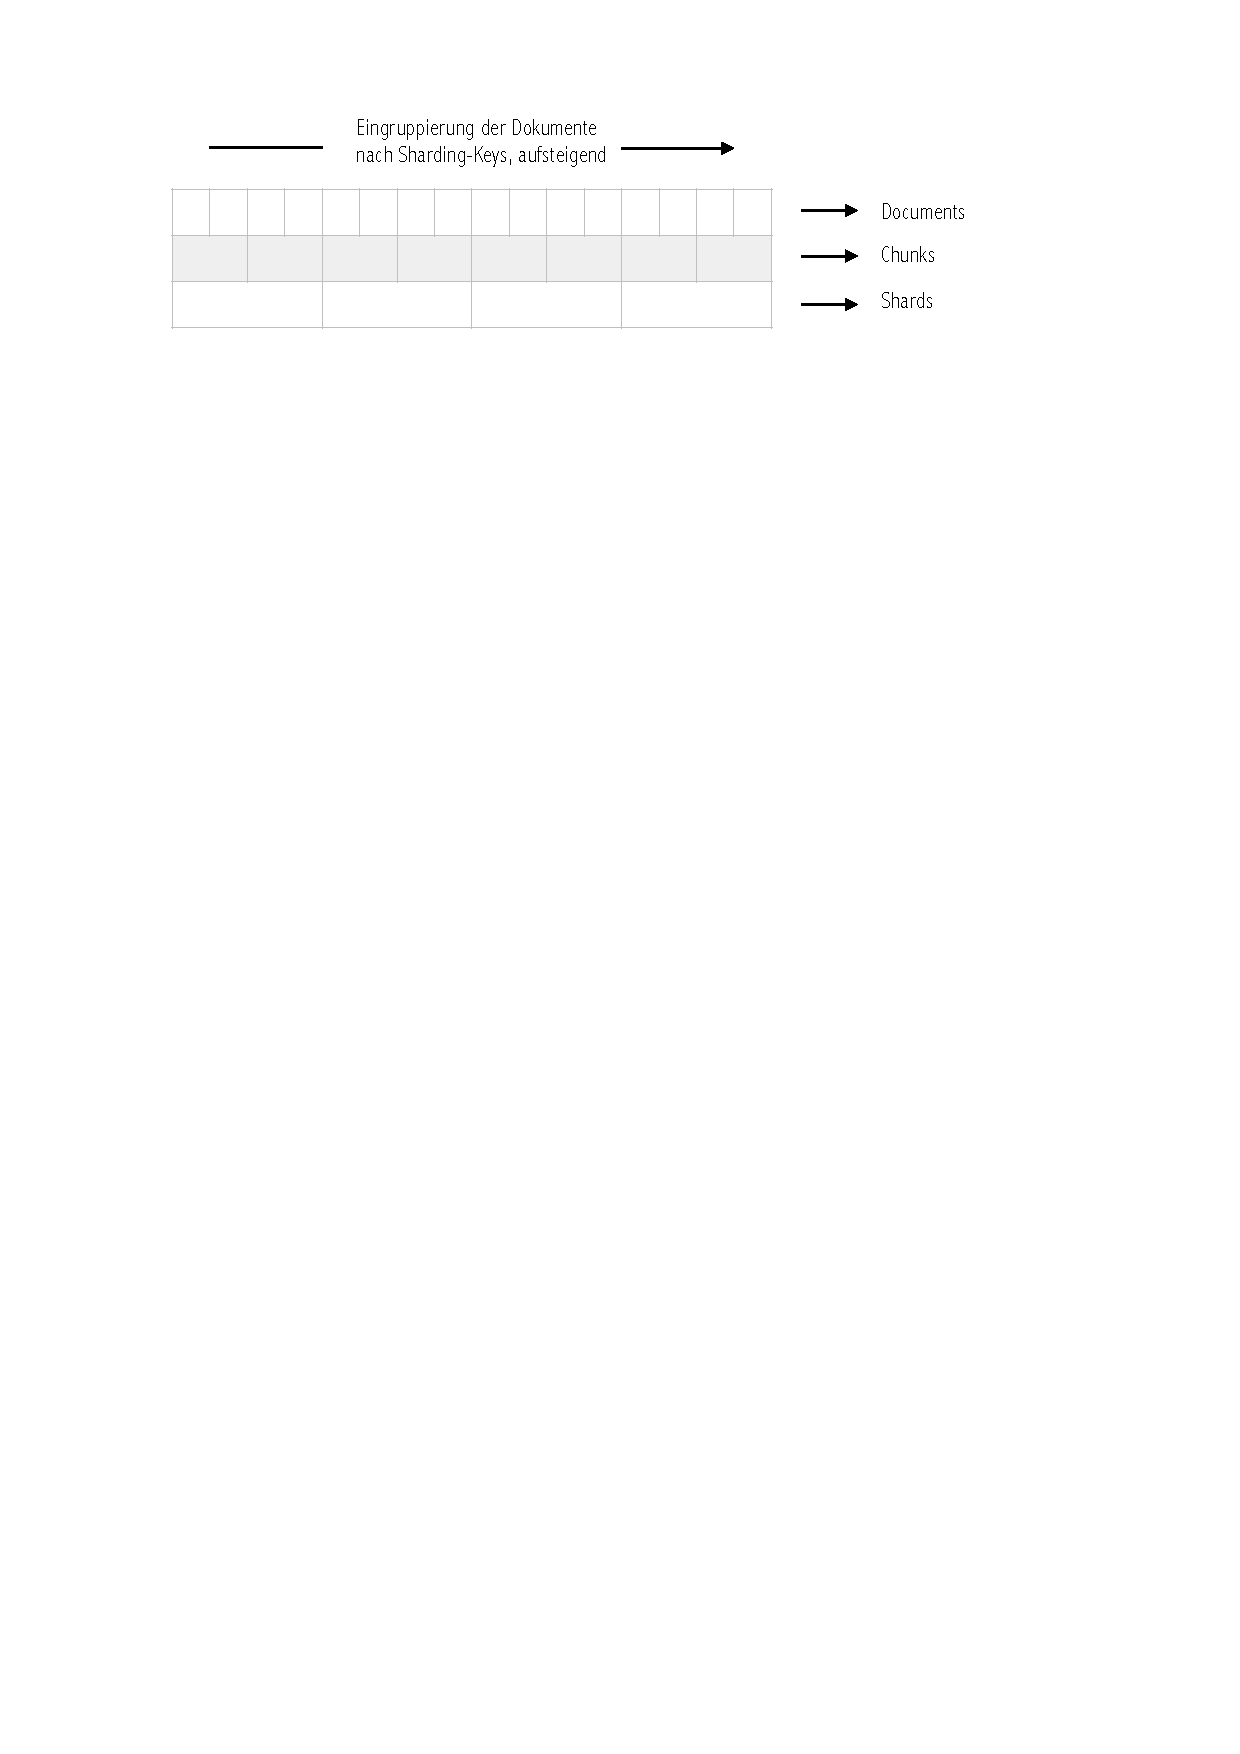
\includegraphics[trim = 25mm 240mm 40mm 20mm, clip, width=0.9\textwidth]{resources/replicaSet/sharding-keys}
\caption[Anordnung der Dokumente in Blocks (=\textit{Chunks}) unter Verwendung des \textit{Shard-Keys}. Mehrere Blocks bilden dementsprechend eine \textit{Shard}.]{Anordnung der Dokumente in Blocks (=\textit{Chunks}) unter Verwendung des \textit{Shard-Keys}. Mehrere Blocks bilden dementsprechend eine \textit{Shard}.}
\label{img:shardKeys}
\end{figure}

Bei der \textit{Shard-Keys} Konfiguration müssen folgende \textit{Constraints\footnote{Introduction to Sharding: \url{https://www.mongodb.com/presentations/back-to-basics-4-introduction-to-sharding?p=589c5c940aca4c55041426f1&utm_campaign=Int_WB_Back\%20to\%20Basics\%20Series\%20\%28English\%29_01_17_EMEA\%20-\%20Follow\%20Up\%204&utm_medium=email&utm_source=Eloqua}, zugegriffen am 2. Februar 2017}} berücksichtigt werden:
\begin{itemize}
\item \textit{Shard-Keys} sind unabänderlich
\item \textit{Shard-Keys} verfügen über eine hohe Kardinalität
\item \textit{Shard-Keys} sind eindeutig
\item \textit{Shard-Keys} existiert dann in jedem Dokument
\item \textit{Shard-Keys} ist bis zum 512 bytes limitiert
\item \textit{Shard-Keys} ist es nicht möglich, als Multi-Key zu bilden
\end{itemize}

\subsection{\colorbox{green}{Replikation (Replication)}}\label{replication}
%\subsection{Replikation (Replication)}\label{replication}
Manchmal kann es dazu kommen, dass ein Server ausfällt und die Schreib- und Lesezugriffe dadurch auf eine kurze Zeit nicht mehr möglich sind. Um Schreib- und Lesezugriffe auch im Fall eines Serverausfalles ständig ermöglichen zu können, hat \mongo\ einen Replikationsmechanismus entwickelt. Der Replikationsmechanismus dient zur Replikation bzw. zum Spiegeln der Daten auf mehreren Servern und funktioniert nach einem \textit{Master-n-Slaves-Prinzip.}
\begin{figure}[H]
   \begin{subfigure}[t]{0.49\textwidth}\vspace{0pt}
   \centering
      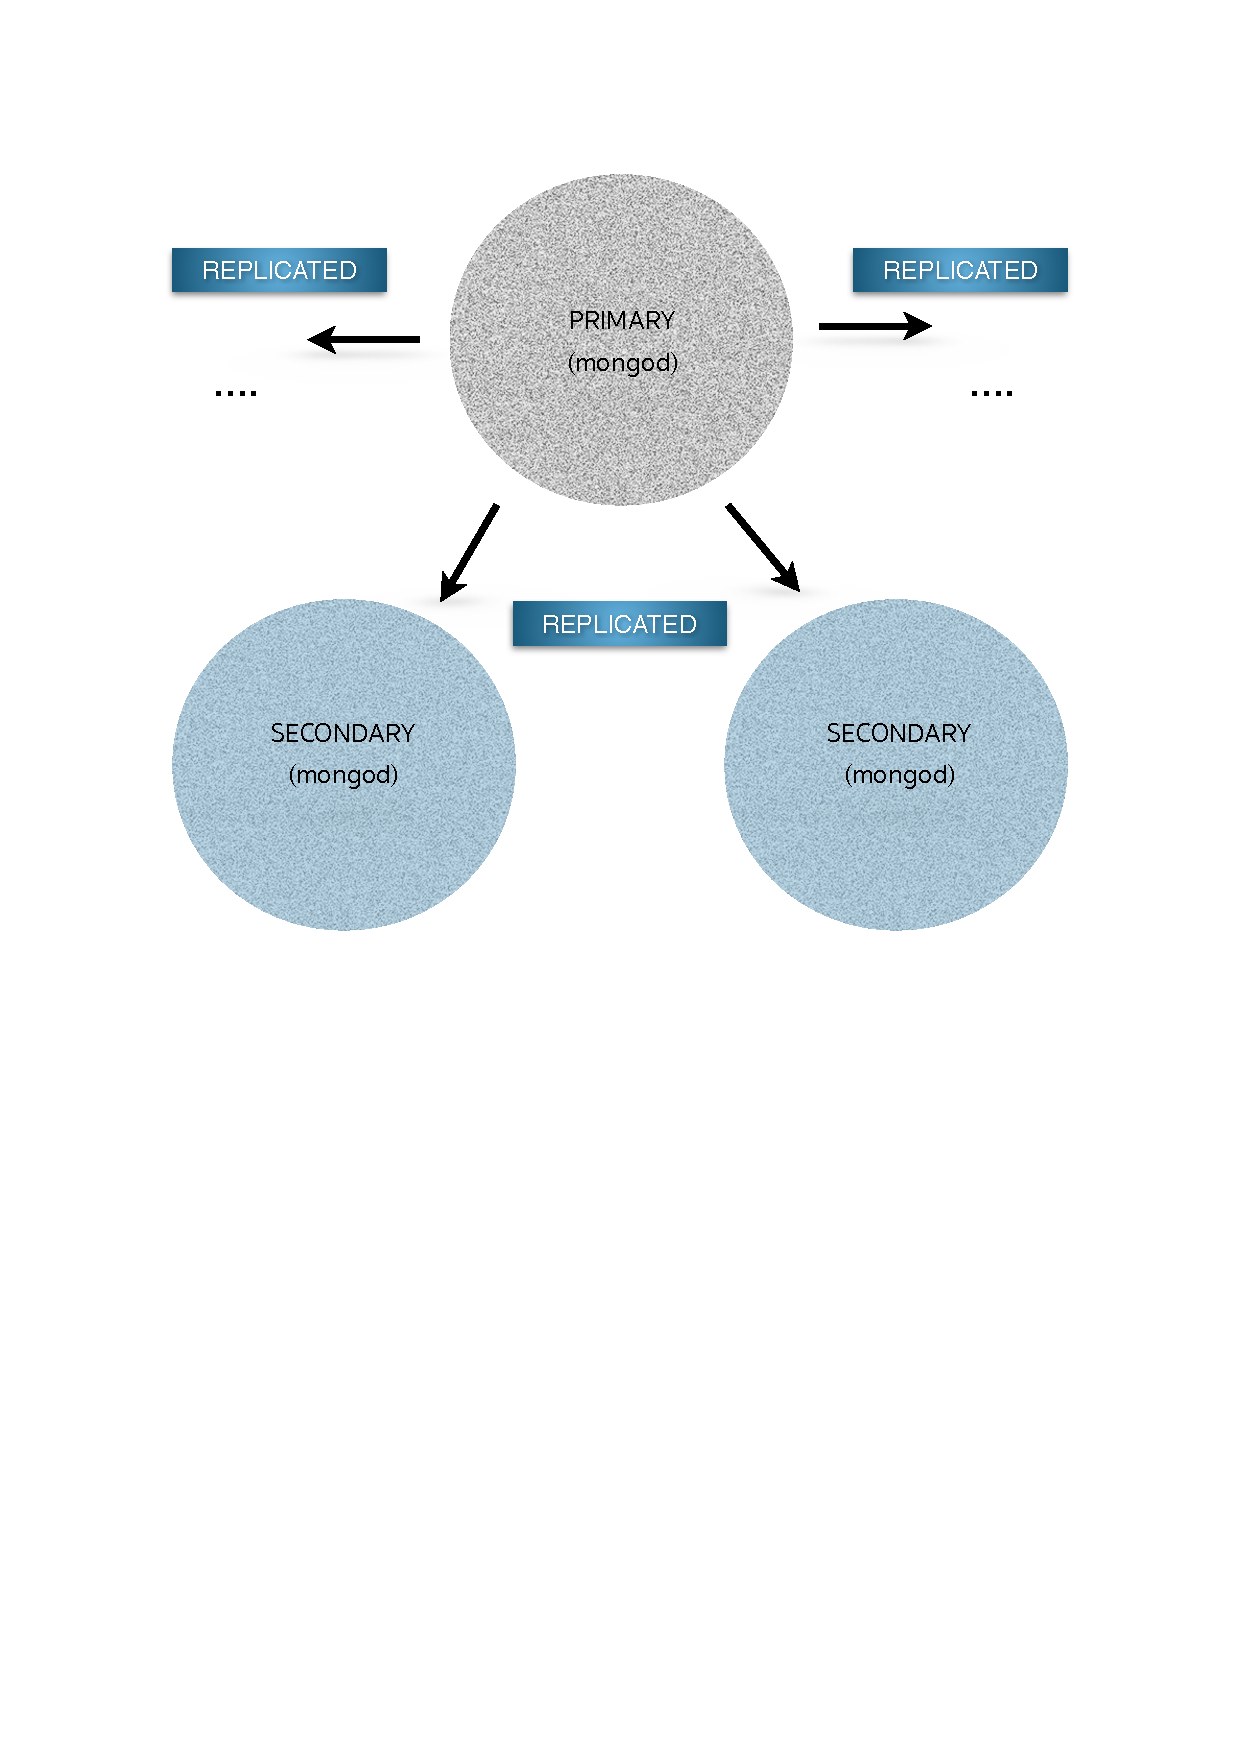
\includegraphics[trim = 28mm 139mm 28mm 29mm, clip, width=0.9\textwidth]{resources/replicaSet/createReplicaSet2}
      \caption[Initialer Zustand des Replica Sets]{Initialer Zustand des Replica Sets}
      % \caption[Ein Beispiel für eine Replikationsgruppe]{Ein Beispiel für eine Replikationsgruppe}
      \label{img:createReplicaSet}
   \end{subfigure}\hfill%
   \begin{subfigure}[t]{0.49\textwidth}\vspace{0pt}
   \centering
      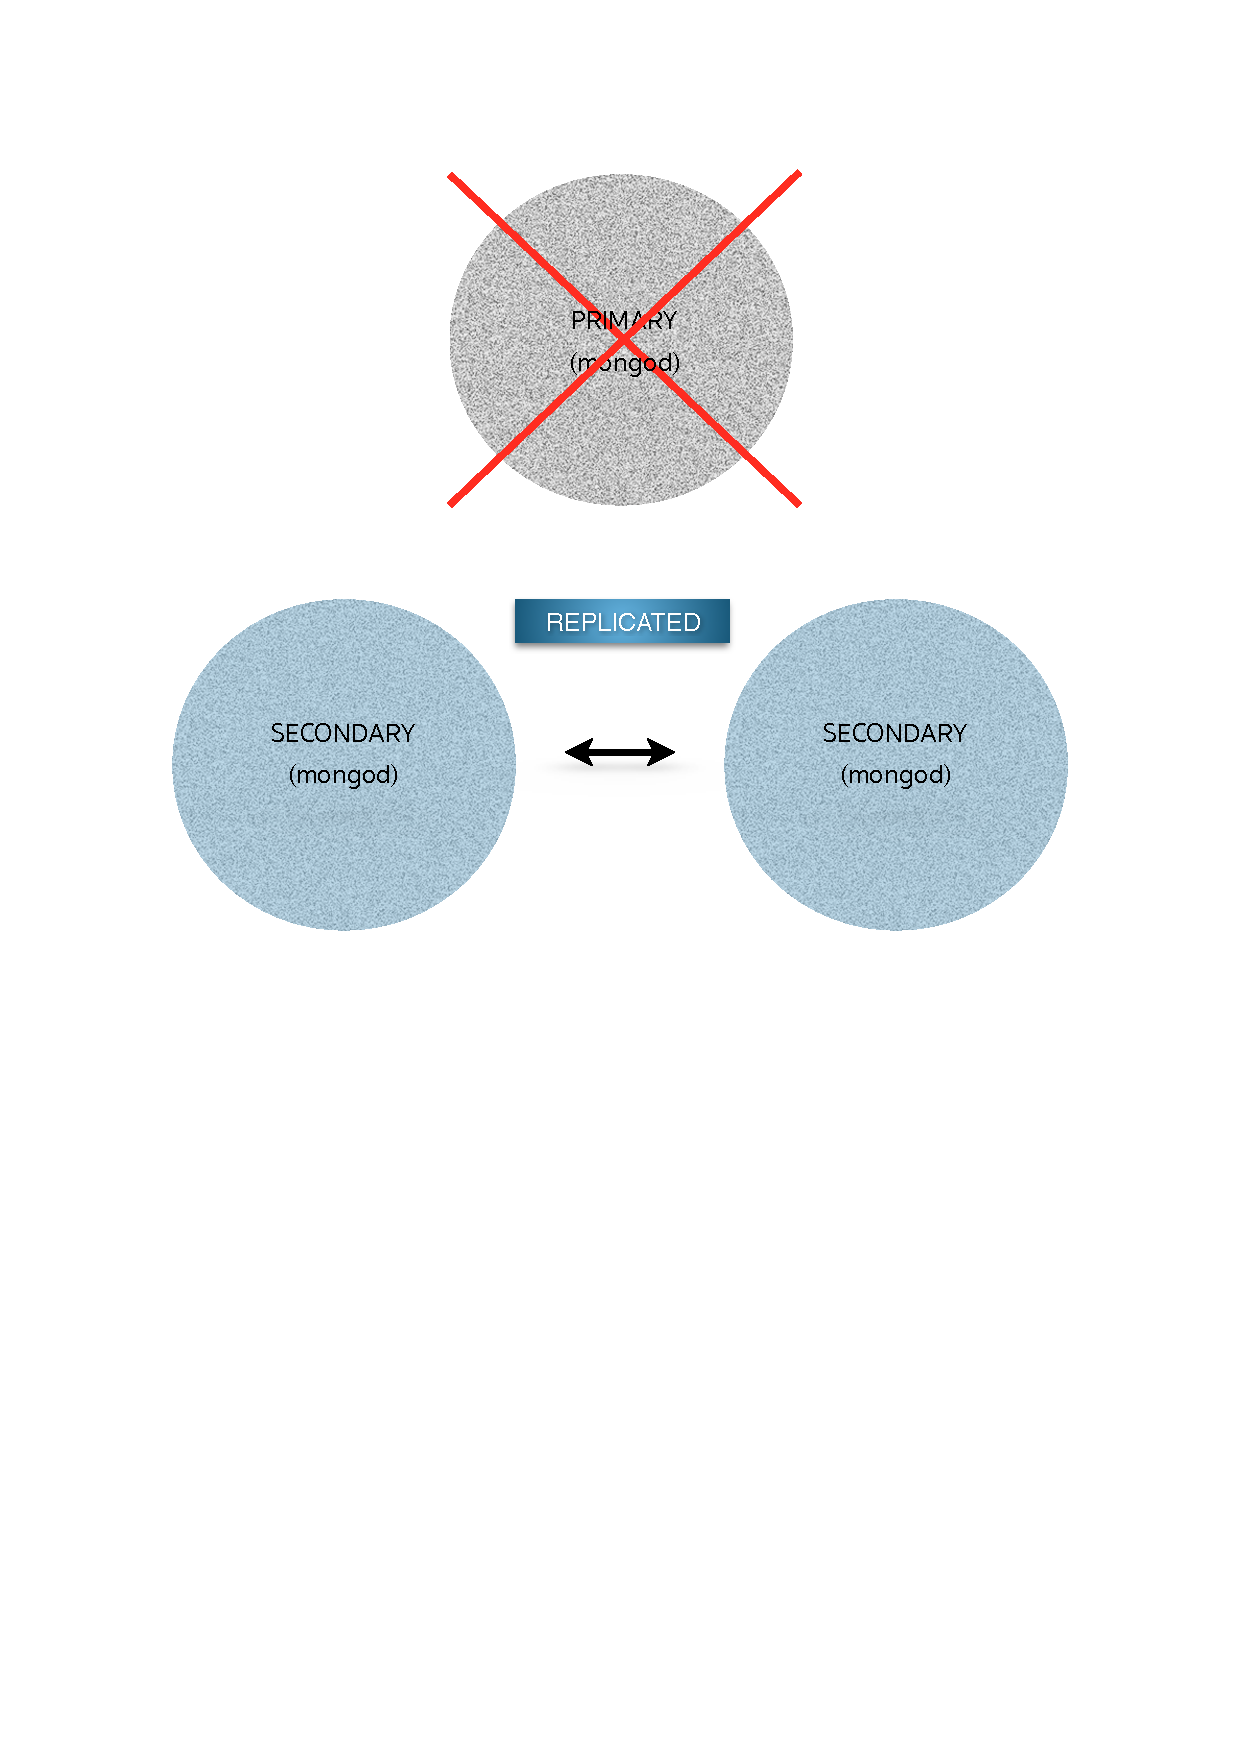
\includegraphics[trim = 28mm 139mm 28mm 29mm, clip, width=0.9\textwidth]{resources/replicaSet/selectNewPrimary}
     \caption[Ausfall des \textbf{Primary}-Knotens]{Ausfall des \textbf{Primary}-Knotens}
      \label{img:selectNewPrimary}
   \end{subfigure}\\[5pt]%
   \centering
   \begin{subfigure}[t]{0.49\textwidth}\vspace{0pt}
   \centering
        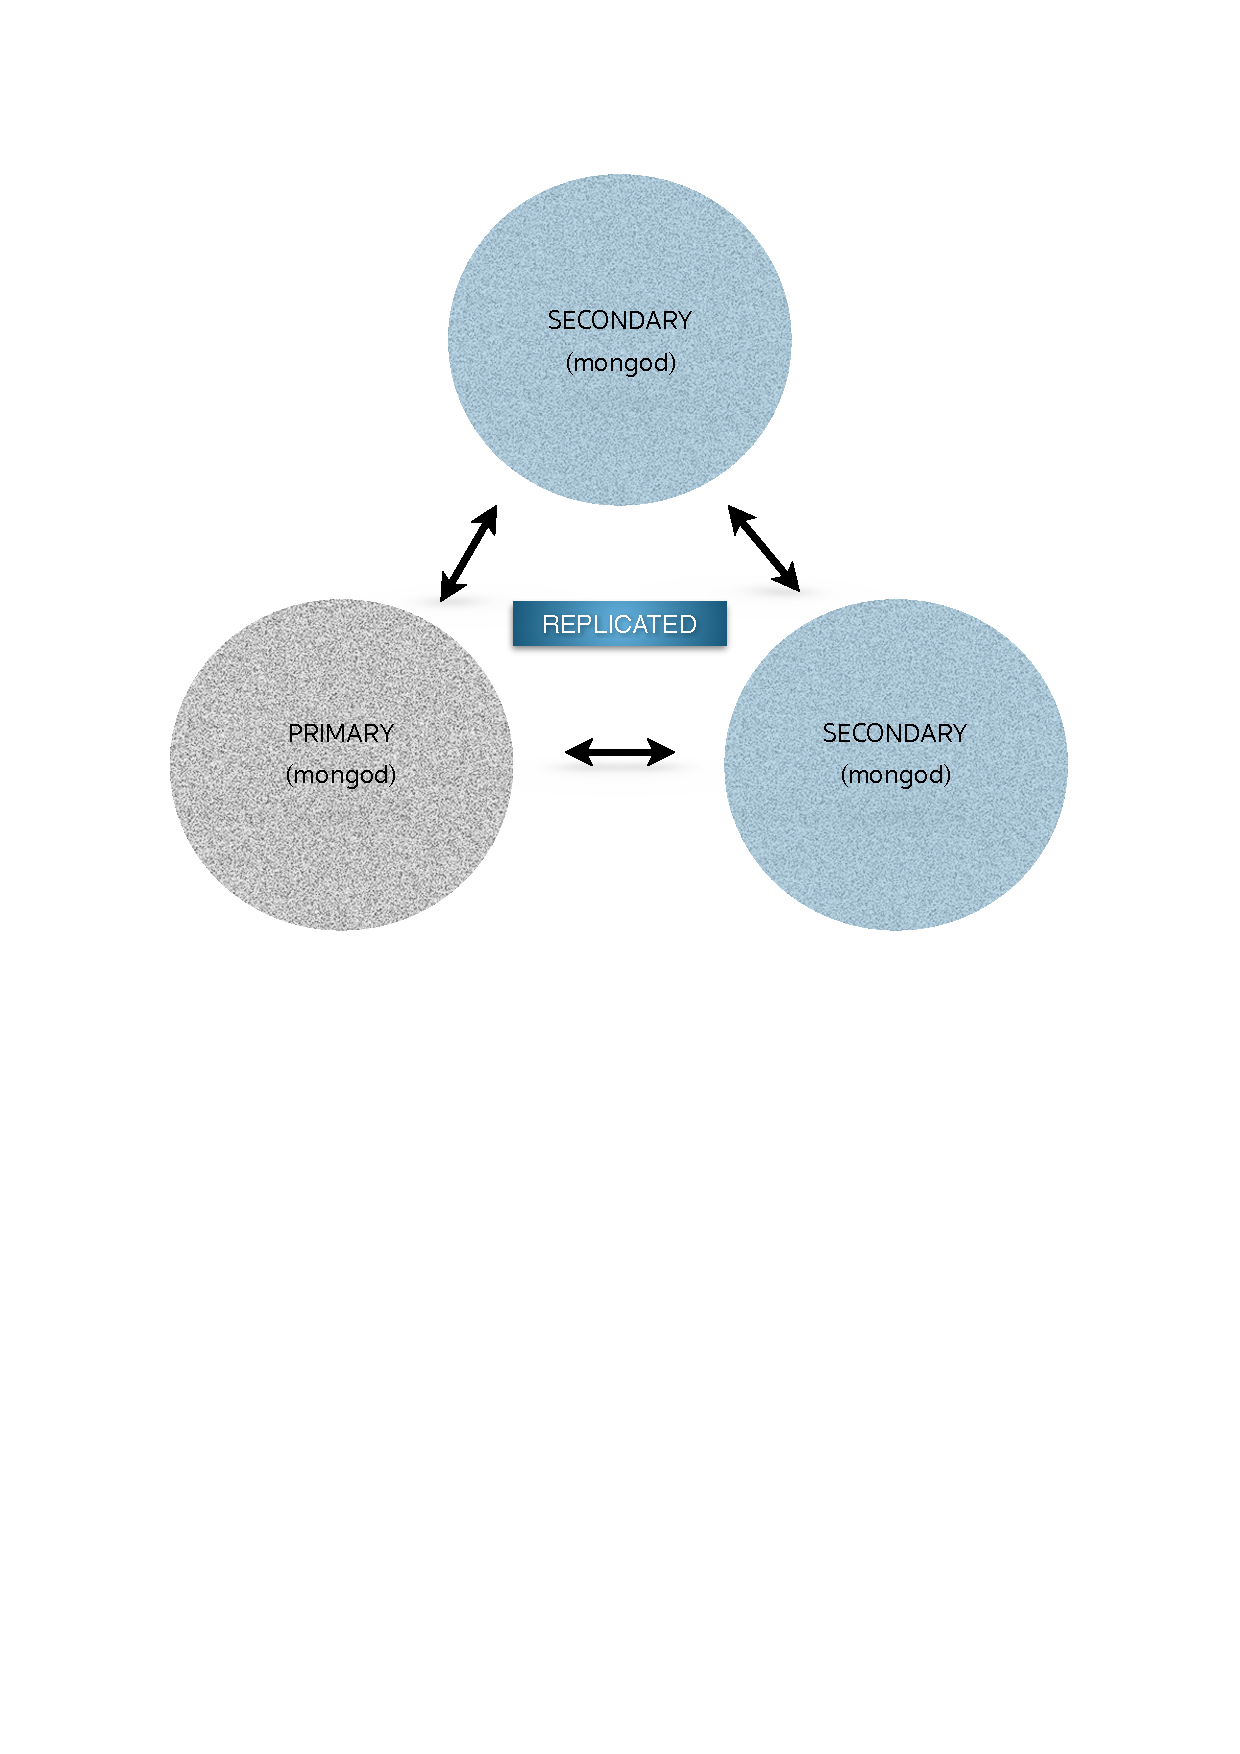
\includegraphics[trim = 28mm 139mm 28mm 29mm, clip, width=0.9\textwidth]{resources/replicaSet/newReplicaSet}
      \caption[Neuer \textbf{Primary} wurde gewählt]{Neuer \textbf{Primary} wurde gewählt}
      \label{img:newReplicaSet}
   \end{subfigure}
   \caption{Szenario für eine Replikationsgruppe mit drei Servern in einer \textit{Shard}}
   \label{img:replicaSetSzenario}
\end{figure}
Ein \textit{Master}, auch ein \textit{Primary} genannt, besitzt Schreib- und Leserechte. Dieser repliziert die Daten auf \textit{n-Slaves}, die auch als \textit{Secondaries} bezeichnet werden. Ein \textit{Primary} mit \textit{n-Secondaries} bilden gemeinsam eine \textit{Shard}. Eine \textit{Shard} kann aus mind. einem Server bestehen. Falls eine \textit{Shard} aus mehreren Servern besteht, so kann \mongo\ die Server in Replikationsgruppe \textit{(Replica set)} anordnen, damit bei Ausfall eines Servers die Verfügbarkeit der Datenbank trotzdem gewährleistet ist. Mit Replikationsgruppen will \mongo\ die Ausfallsicherheit sicherstellen. Die Abbildung \ref{img:replicaSetSzenario} veranschaulicht ein Szenario für eine Replikationsgruppe mit drei Knoten. Jeder Knoten aus der Gruppe ist als einen eigenen Server vorzustellen. Das \textit{Master-n-Slaves-Prinzip} besagt, dass in einer Replikationsgruppe nur ein Master und n-Slaves existieren können, um eine strenge Konsistenz gewährleisten zu können. 
%\begin{figure}[H]
%\centering
%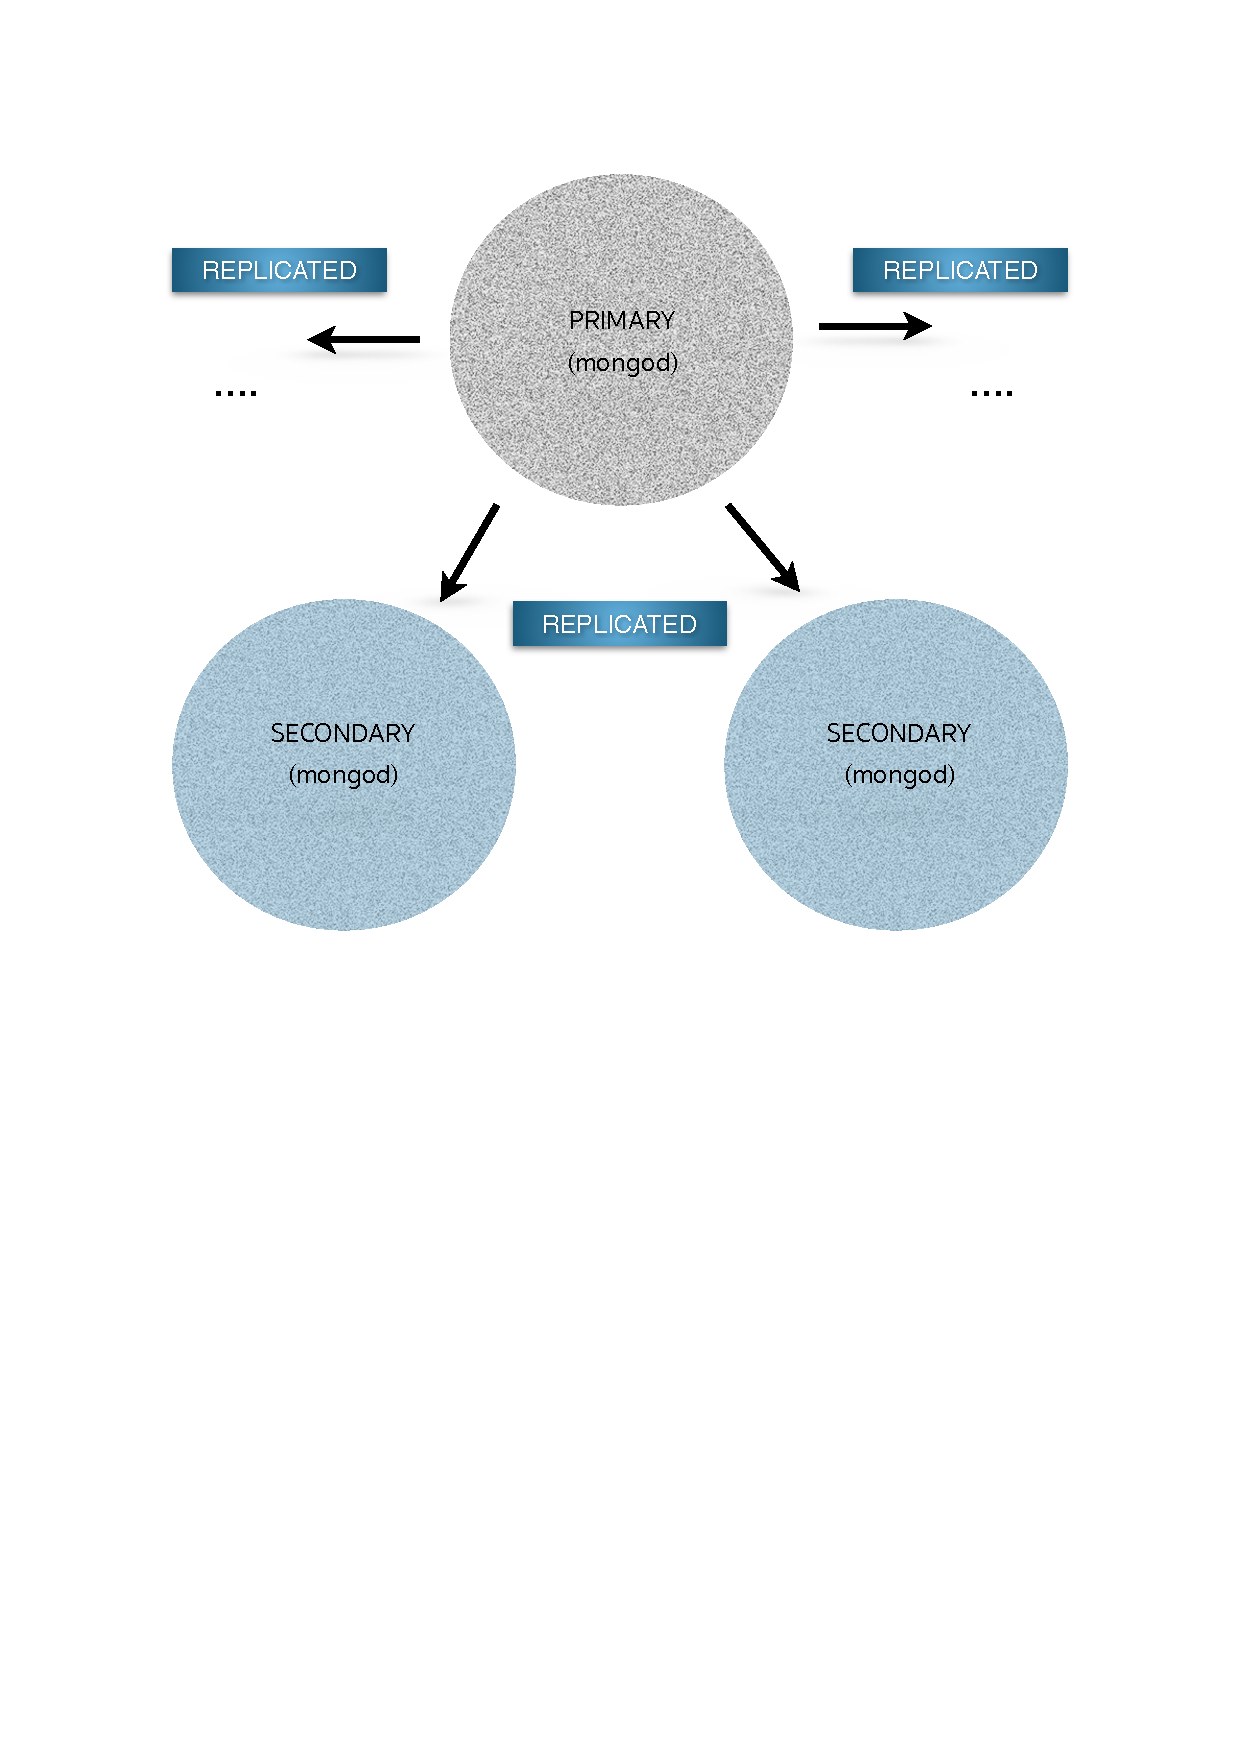
\includegraphics[trim = 0mm 139mm 0mm 28mm, clip, width=0.7\textwidth]{resources/replicaSet/createReplicaSet2}
%\caption[Ein Beispiel für eine Replikationsgruppe]{Ein Beispiel für eine Replikationsgruppe}
%\label{img:createReplicaSet}
%\end{figure}

%\begin{figure}[H]
%\centering
%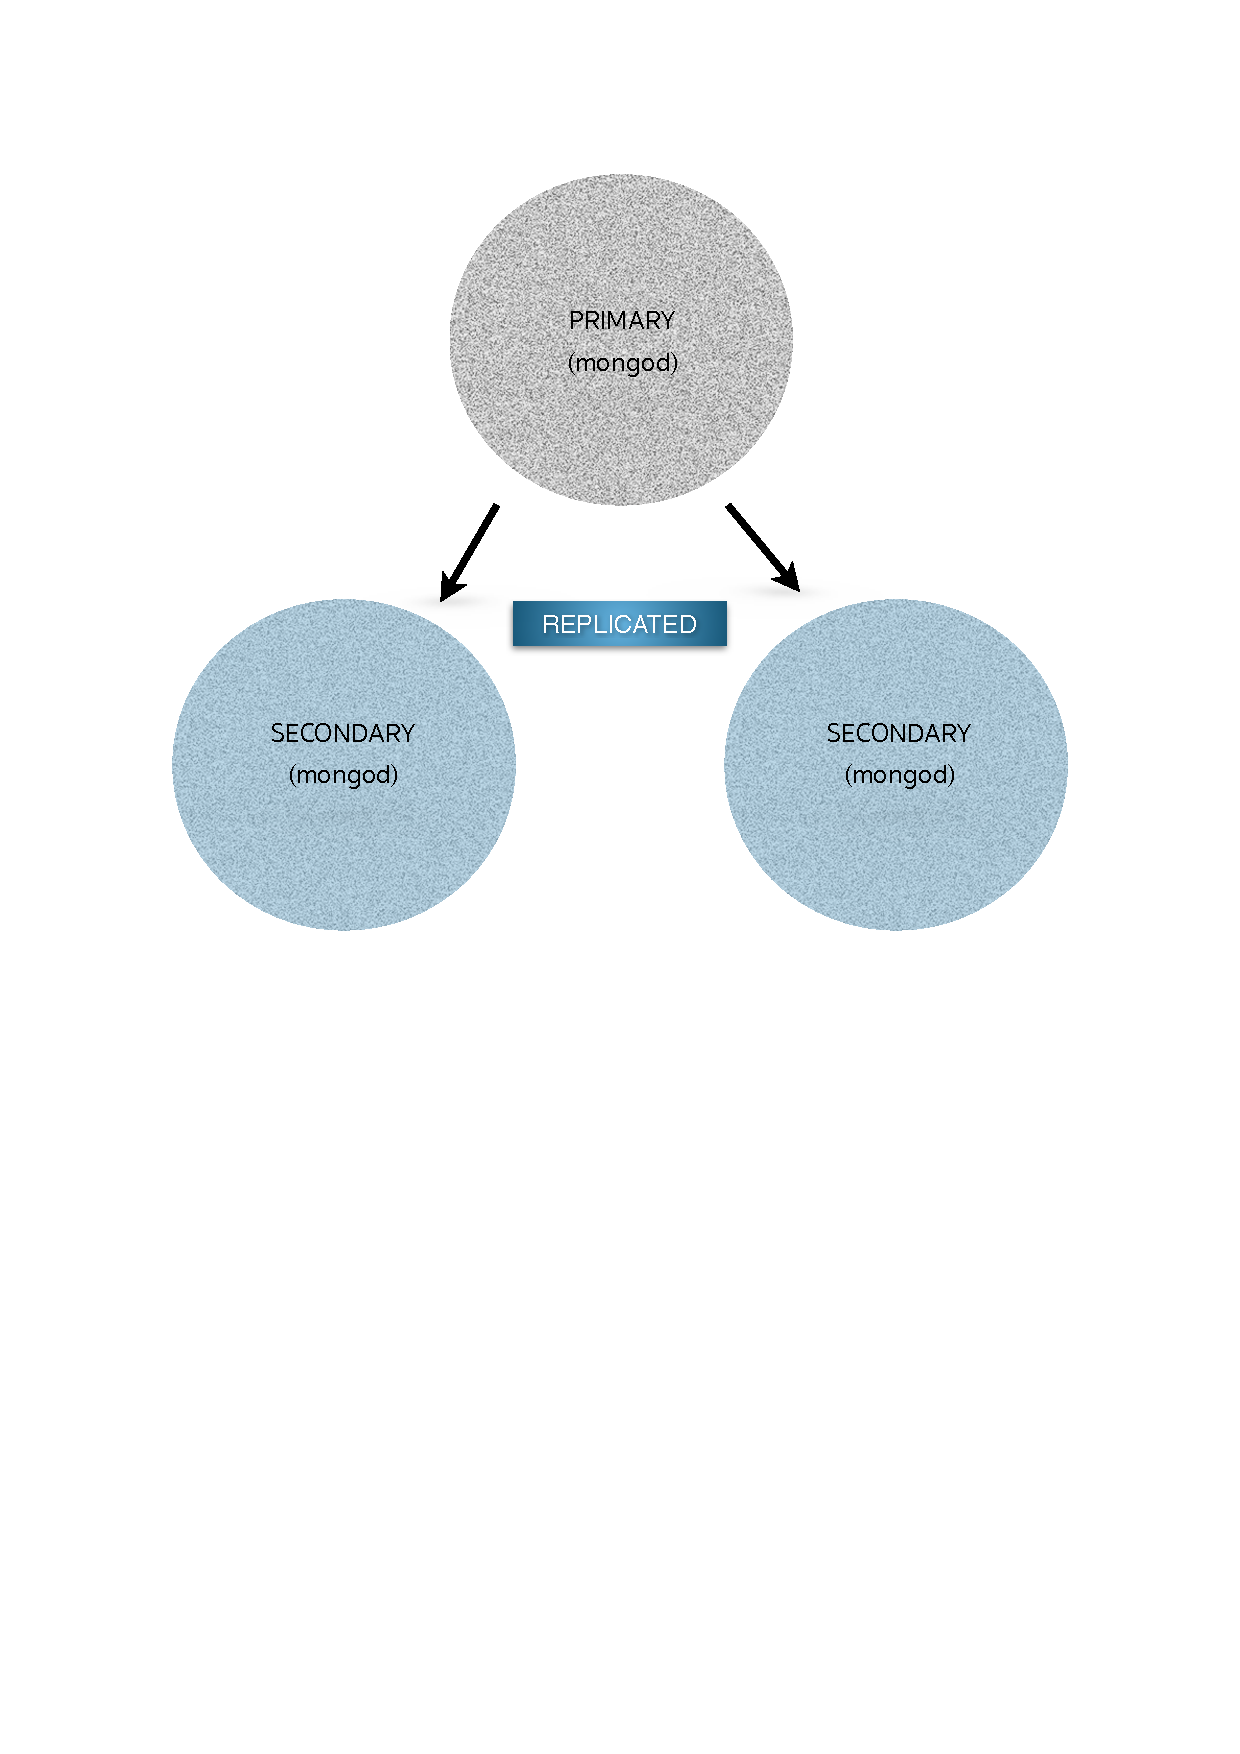
\includegraphics[trim = 0mm 139mm 0mm 9mm, clip, width=0.7\textwidth]{resources/replicaSet/createReplicaSet}
%\caption[Eine Replikationsgruppe mit einem Master und n-Slaves erzeugen]{Eine Replikationsgruppe mit einem Master und n-Slaves erzeugen}
%\label{img:createReplicaSet}
%\end{figure}
\begin{figure}[H]
   \begin{subfigure}[t]{0.49\textwidth}\vspace{0pt}
   \centering
    	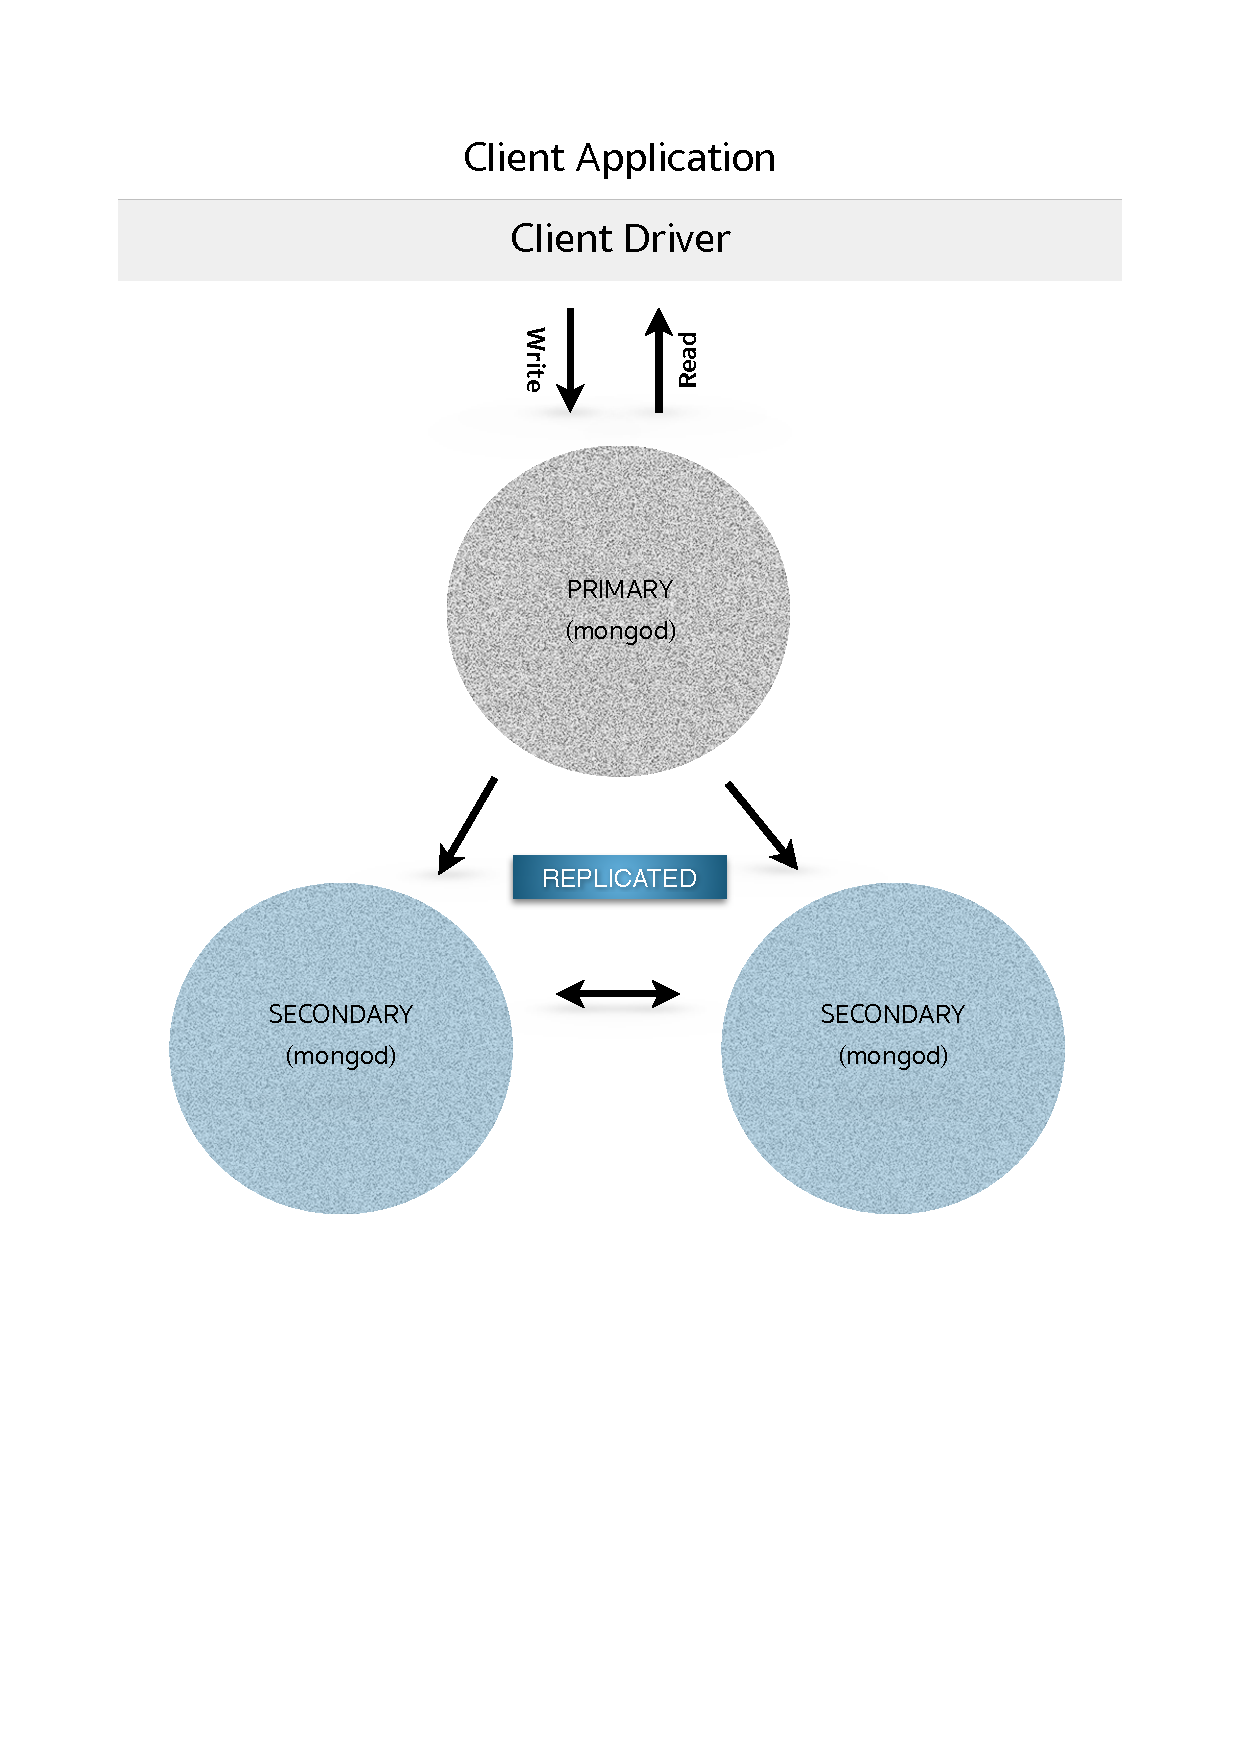
\includegraphics[trim = 0mm 90mm 0mm 20mm, clip, width=1.0\textwidth]{resources/replicaSet/replicaSetStrongConsistency}
	\caption[Lesezugriffe nur über Primary möglich]{Lesezugriffe nur über \textbf{Primary} möglich}
	\label{img:slaveNotOk}
   \end{subfigure}\hfill%
   \begin{subfigure}[t]{0.49\textwidth}\vspace{0pt}
   \centering
	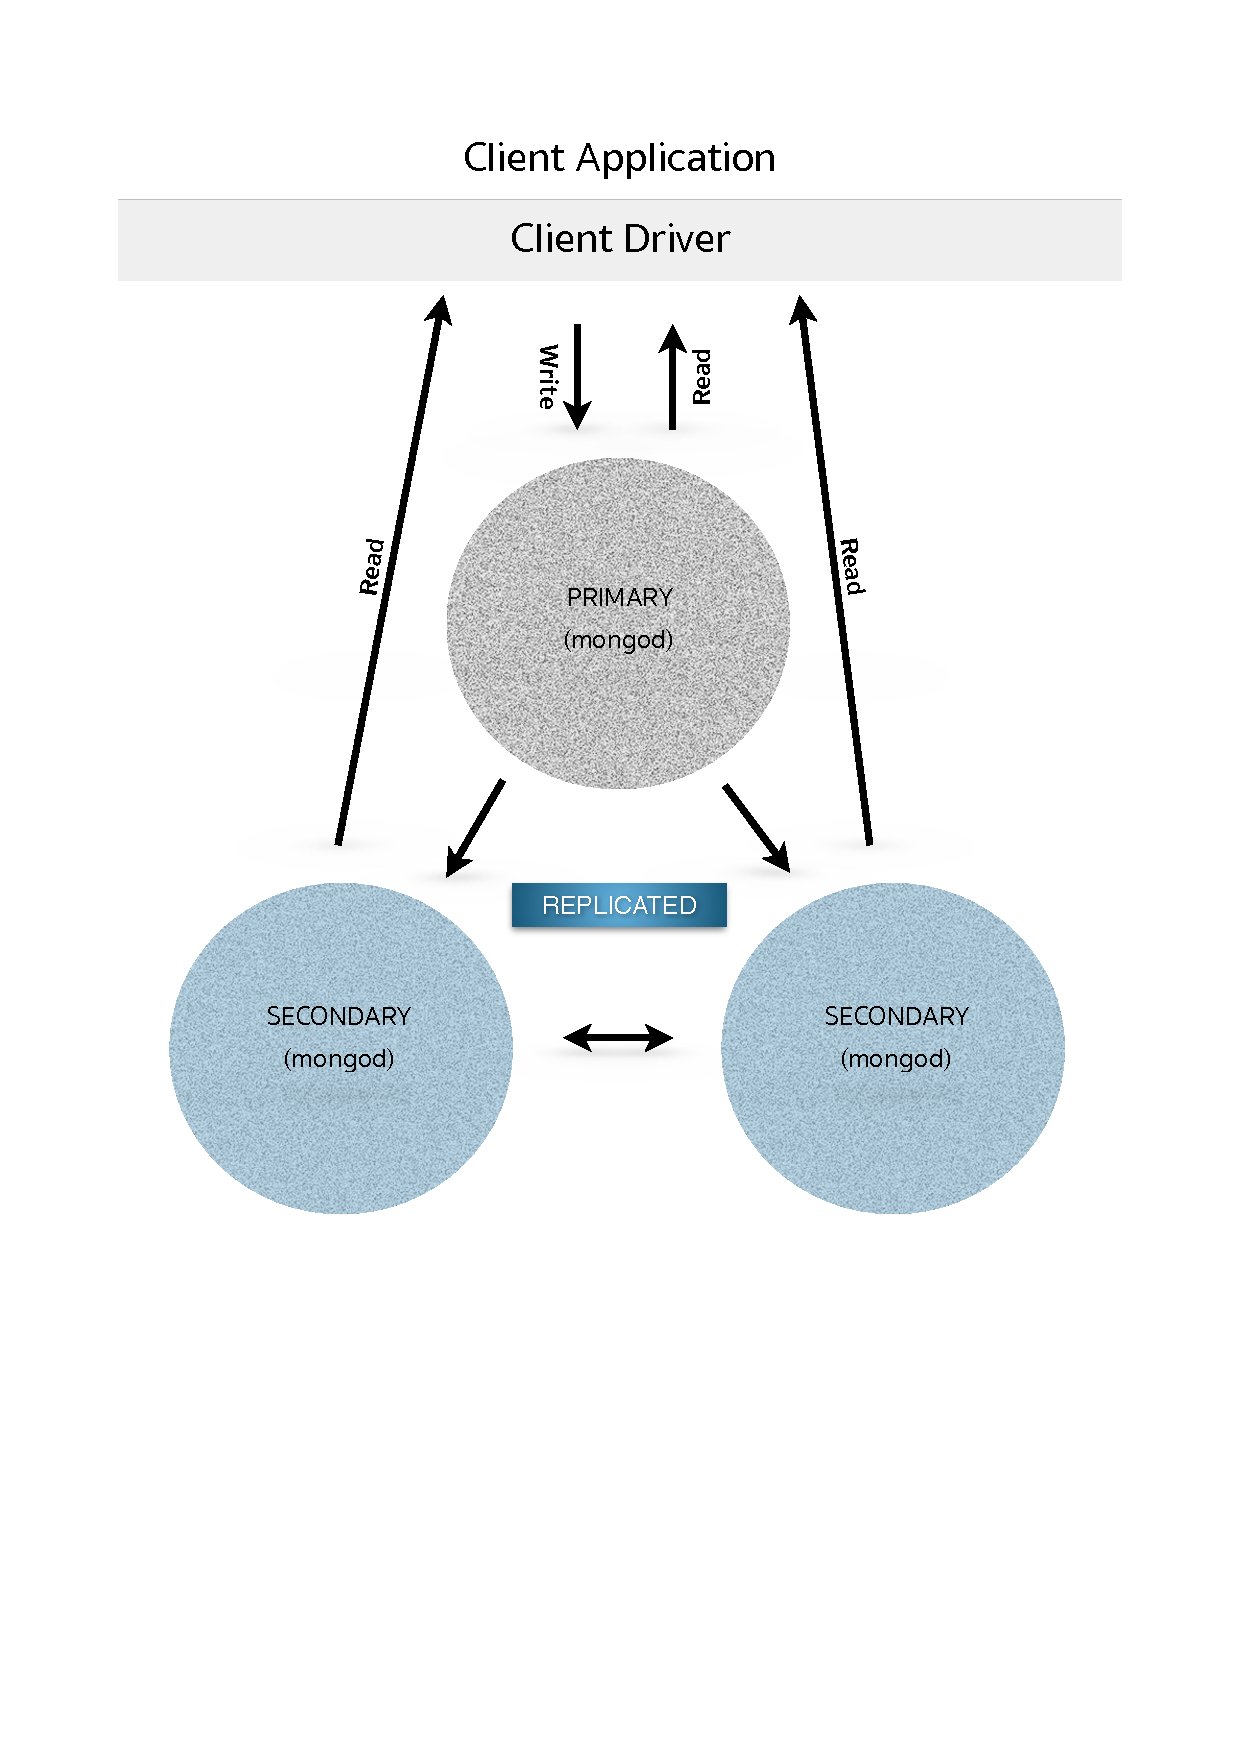
\includegraphics[trim = 0mm 90mm 0mm 20mm, clip, width=1.0\textwidth]{resources/replicaSet/eventualConsistency}
	\caption[Lesezugriffe auch über Secondaries freigeschaltet]{Lesezugriffe auch über \textbf{Secondaries} freigeschaltet}
	\label{img:slaveOk}
   \end{subfigure}\\[5pt]%
   \caption{Freischaltung der Lesezugriffe}
   \label{img:secondariesLowToRead}
\end{figure}
Im Gegenteil zu dem Primary sind bei Secondaries die Schreib- und Leserechte von Anfang an nicht möglich. Falls der Kontext der Anwendung verlangt, können nur die Leserechte entsprechend freigeschaltet werden. 
%\begin{figure}[H]
%\centering
%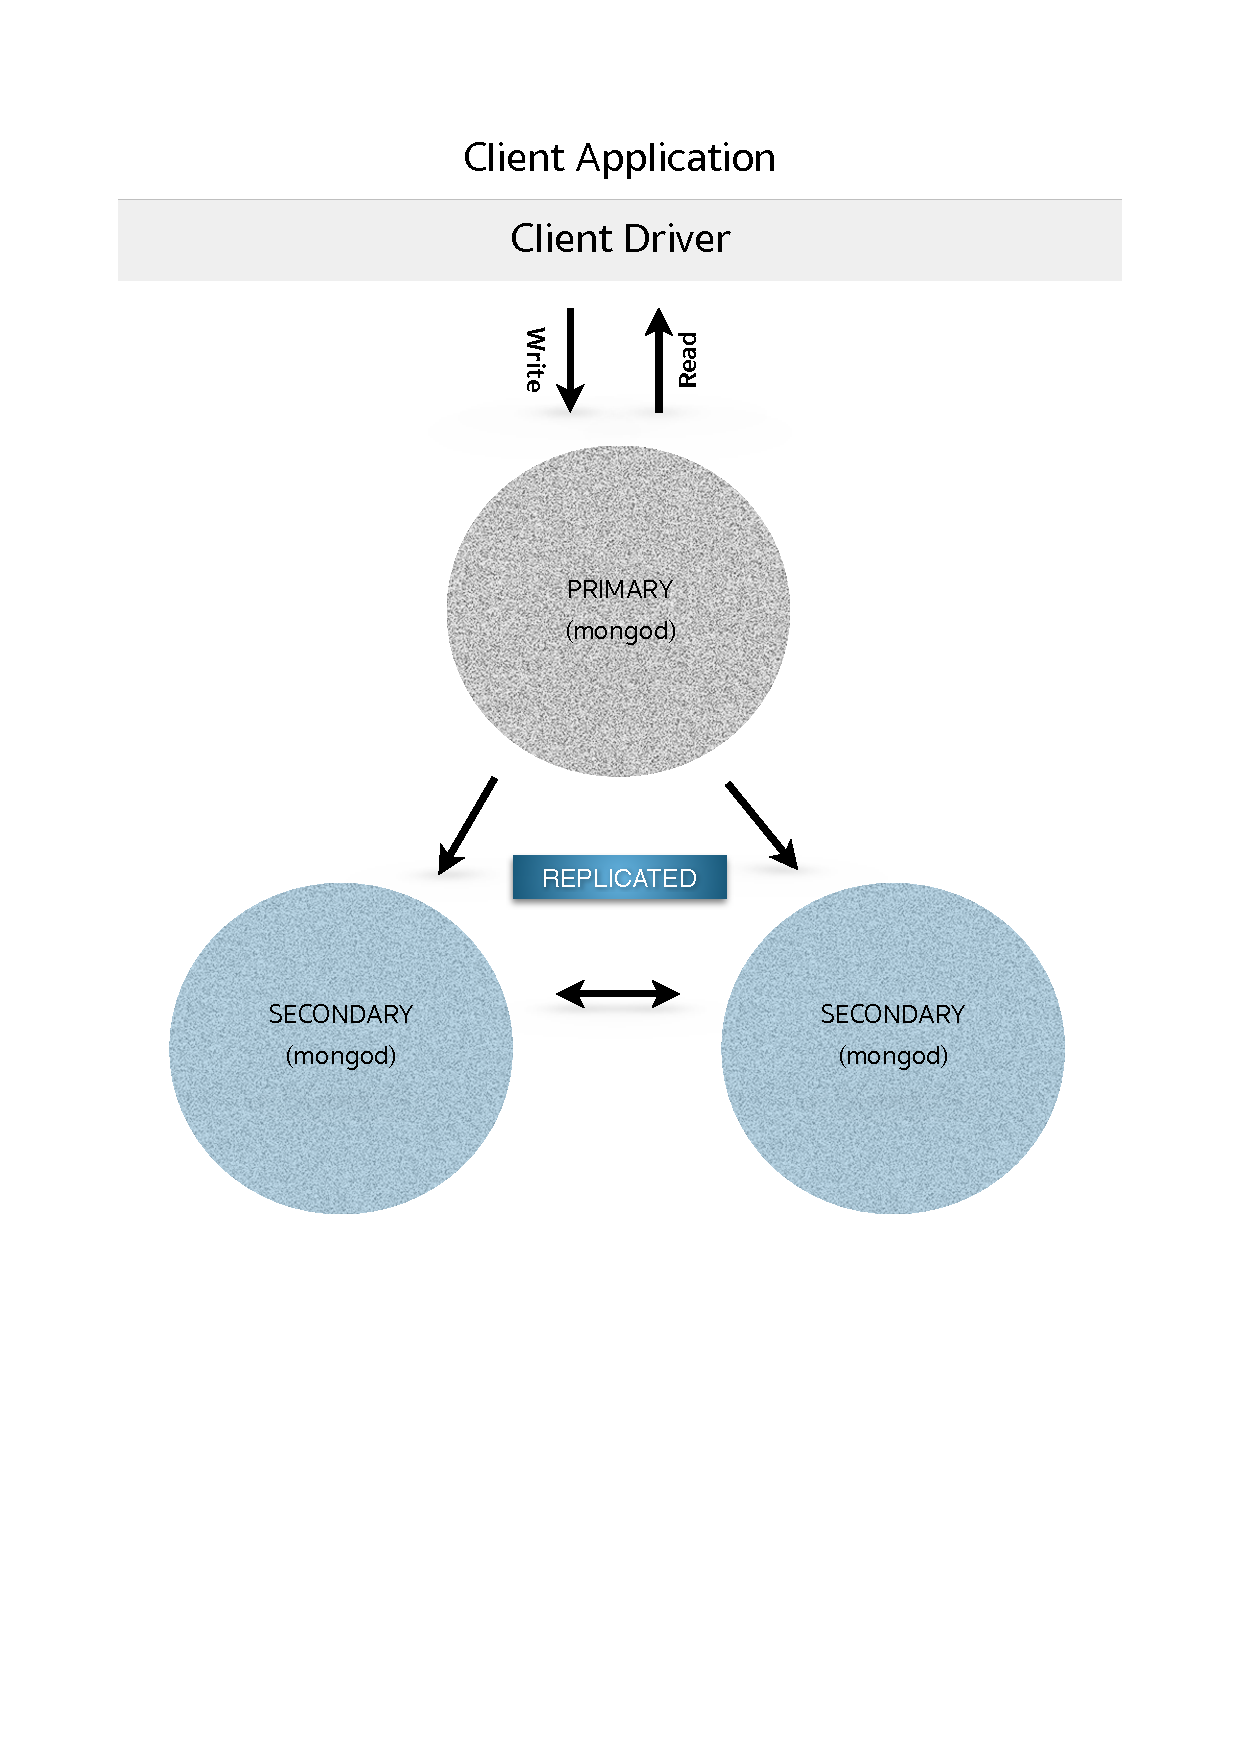
\includegraphics[trim = 0mm 90mm 0mm 20mm, clip, width=0.7\textwidth]{resources/replicaSet/replicaSetStrongConsistency}
%\caption[Lesezugriffe nur über Primary möglich]{Lesezugriffe nur über \textbf{Primary} möglich}
%\label{img:slaveNotOk}
%\end{figure}
%
%\begin{figure}[H]
%\centering
%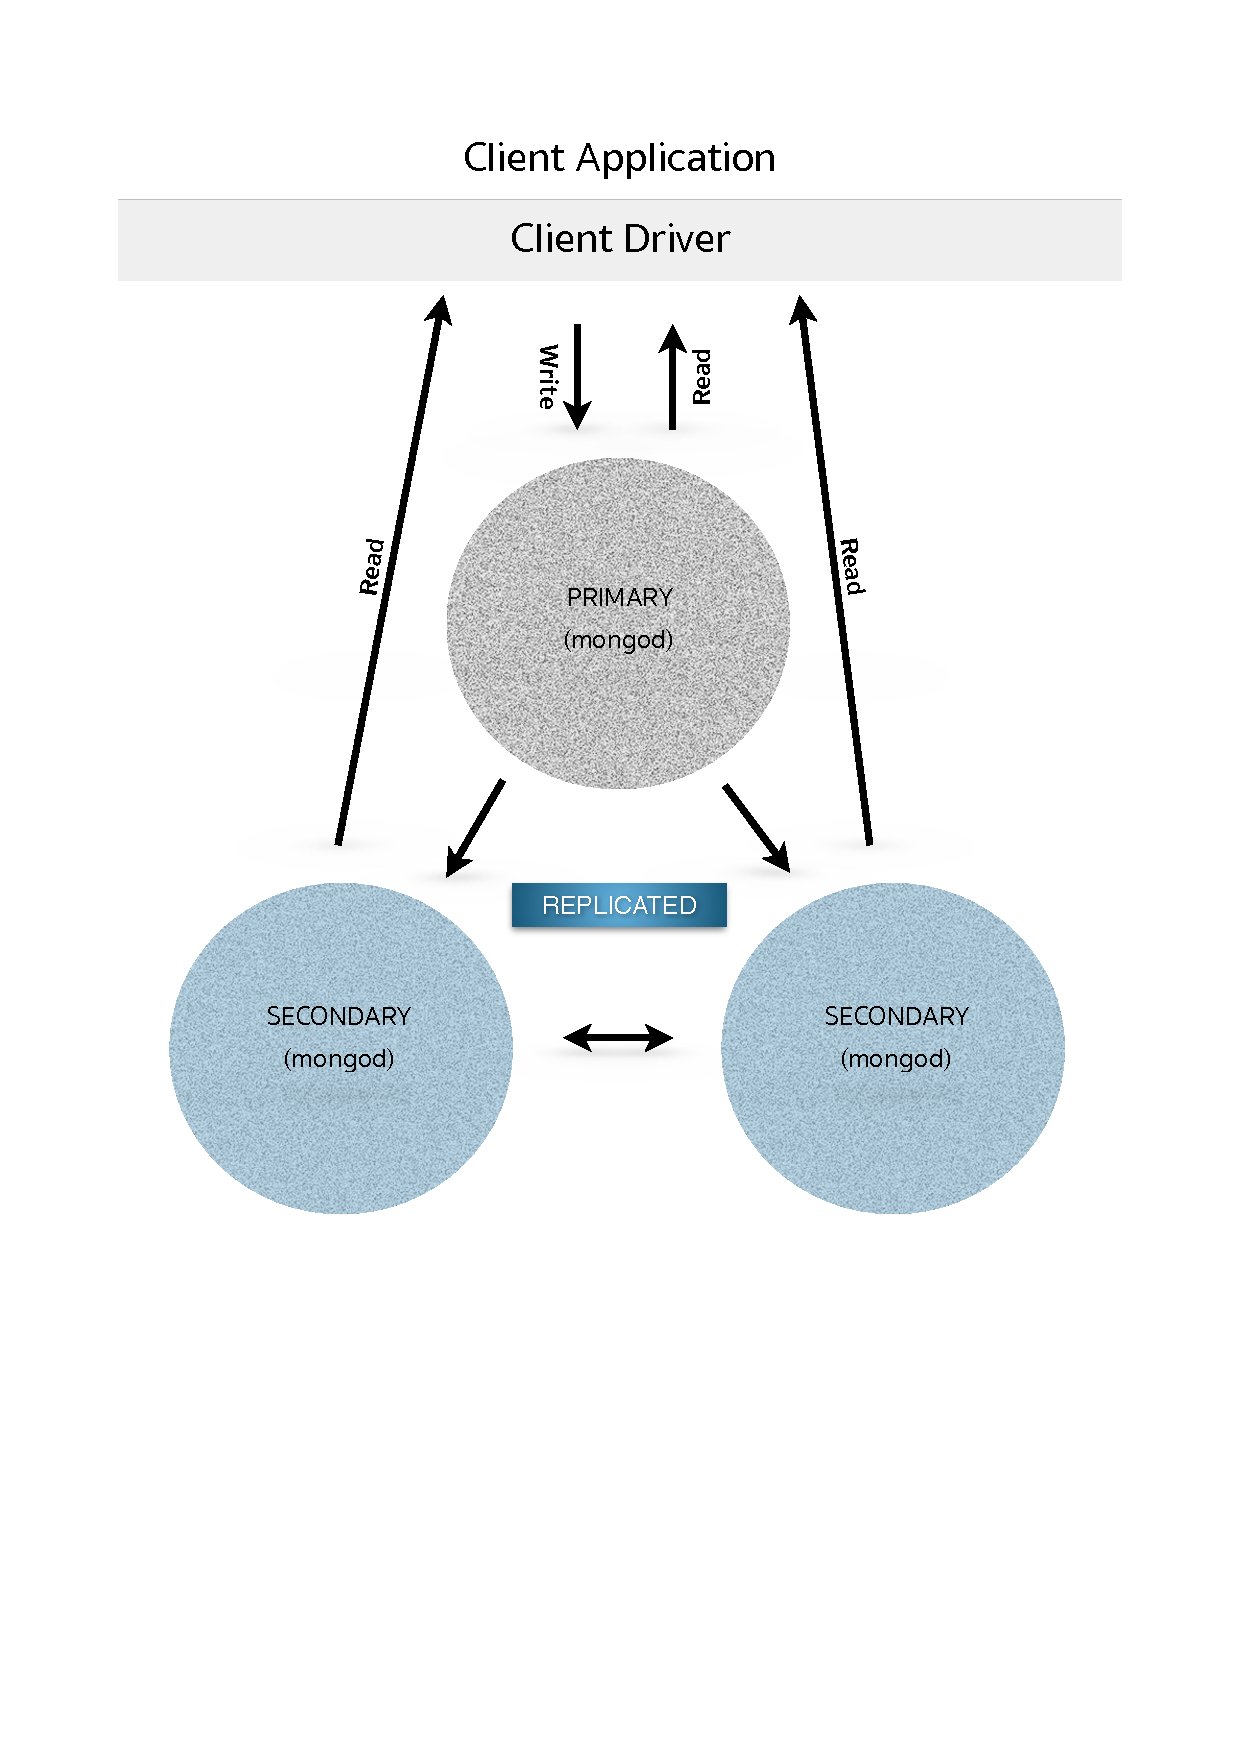
\includegraphics[trim = 0mm 90mm 0mm 20mm, clip, width=0.7\textwidth]{resources/replicaSet/eventualConsistency}
%\caption[Lesezugriffe auch über Secondaries freigeschaltet]{Lesezugriffe auch über \textbf{Secondaries} freigeschaltet}
%\label{img:slaveOk}
%\end{figure}

%\begin{figure}[H]
%\centering
%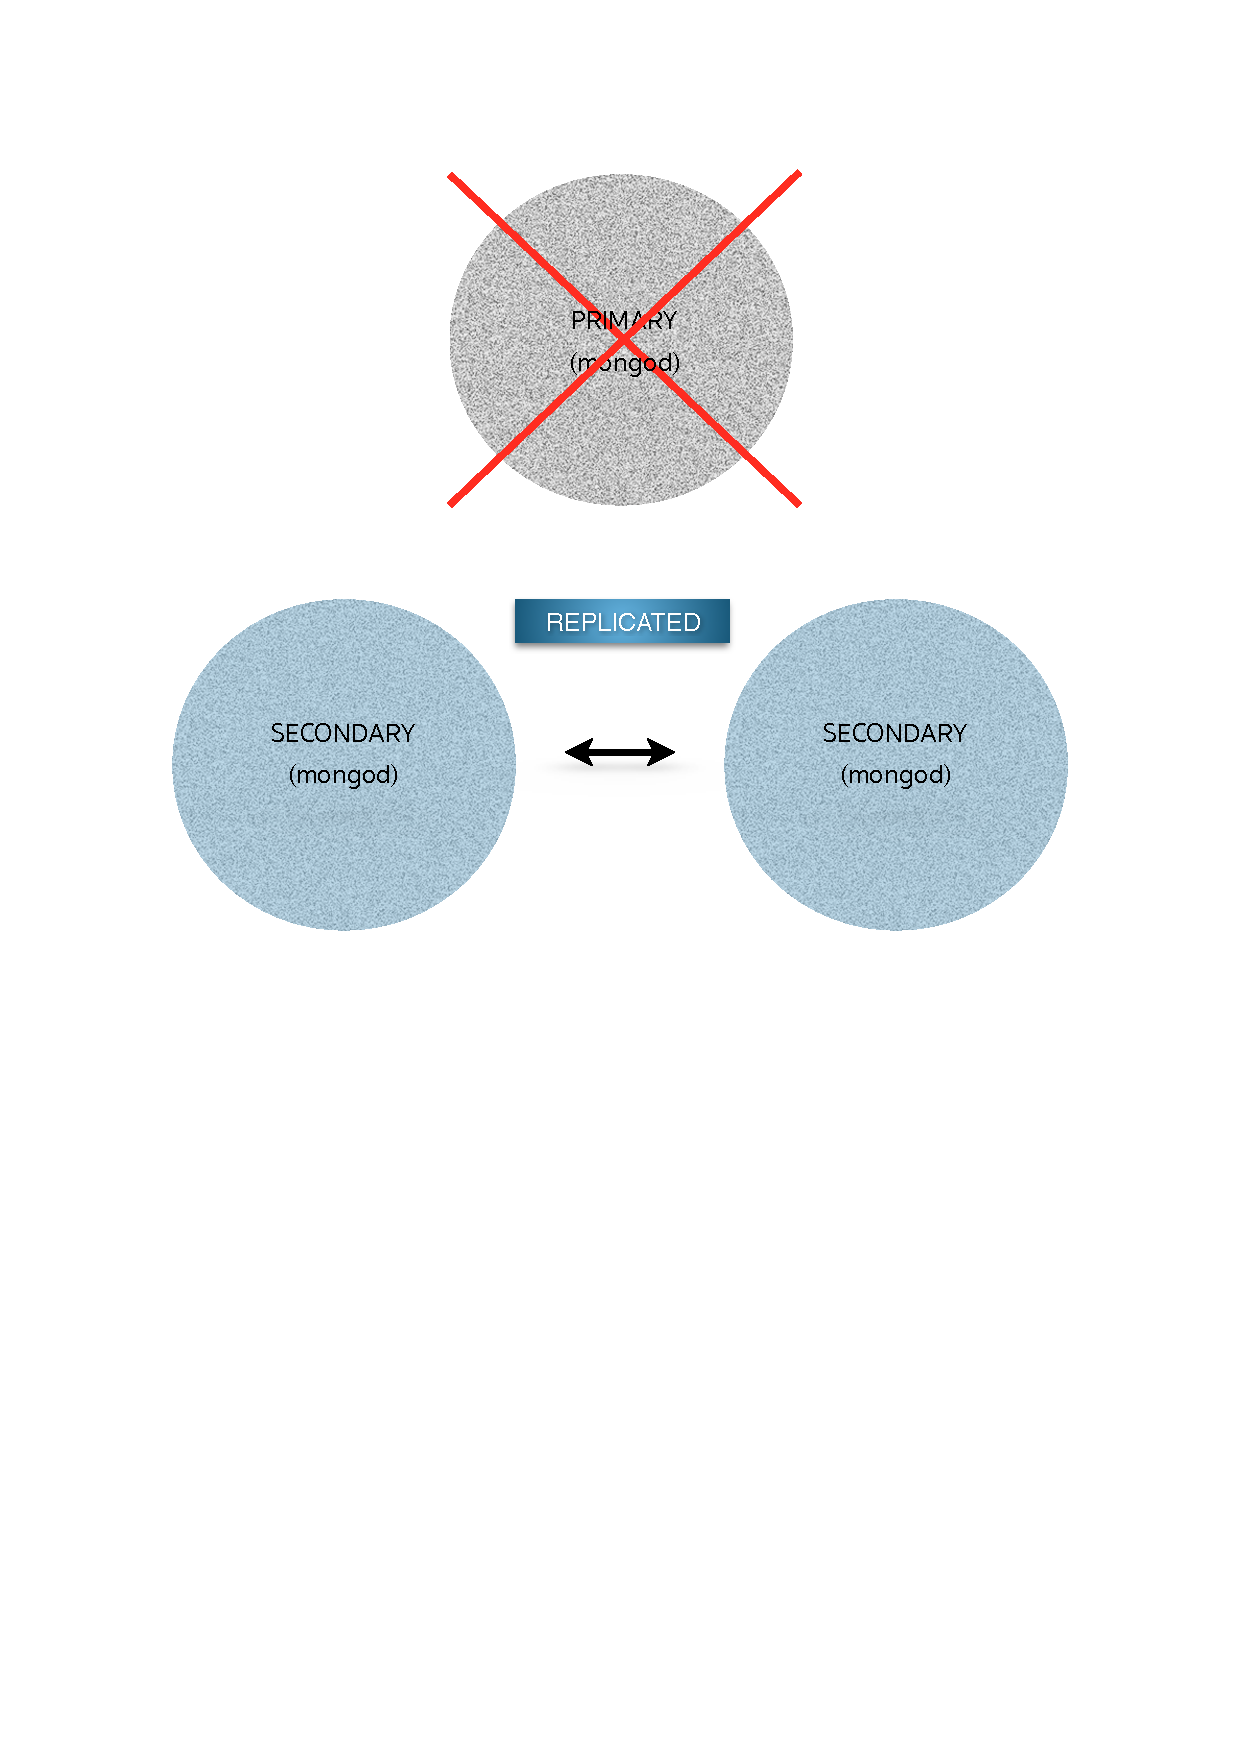
\includegraphics[trim = 0mm 139mm 0mm 28mm, clip, width=0.7\textwidth]{resources/replicaSet/selectNewPrimary}
%\caption[\textbf{Primary} fehlte aus]{\textbf{Primary} fehlte aus}
%\label{img:selectNewPrimary}
%\end{figure}

%\begin{figure}[H]
%\centering
%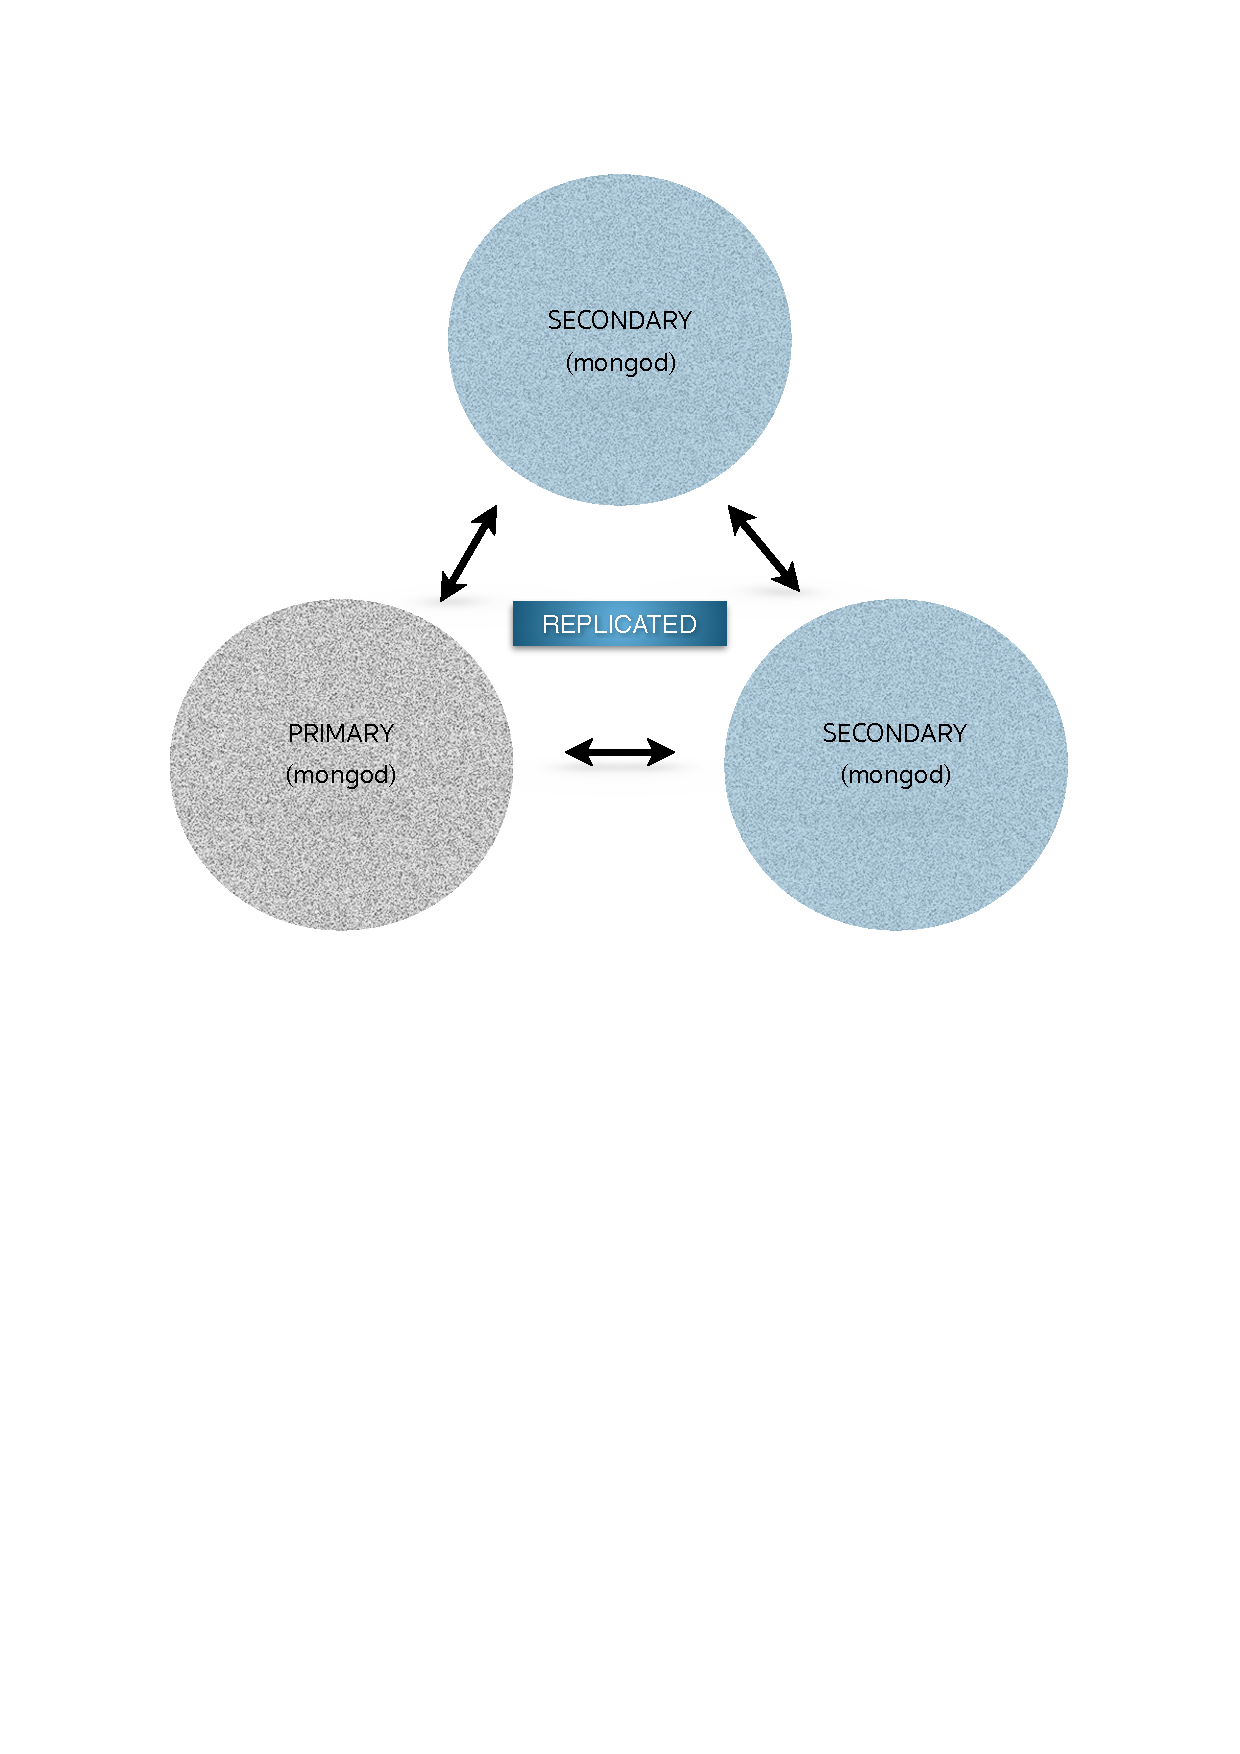
\includegraphics[trim = 0mm 139mm 0mm 28mm, clip, width=0.7\textwidth]{resources/replicaSet/newReplicaSet}
%\caption[Mitglieder der Replikationsgruppe wählten einen neuen \textbf{Primary} aus]{Mitglieder der Replikationsgruppe wählten einen neuen \textbf{Primary} aus}
%\label{img:newReplicaSet}
%\end{figure}
\subsubsection{Eine Replikationsgruppe erzeugen}
In diesem Teilabschnitt wird eine Replikationsgruppe mit insgesamt drei Servern erzeugt. Jeder Schritt der Konfiguration wird in diesem Teilabschnitt nachgespielt.
%
%Über die sog. \textit{Mongo Shell} auf der Kommandozeile ist es möglich,  zum Serverprozess zu verbinden und nötige Schreib- und Lesezugriffe durchzuführen.
%
%Um eine Replikationsgruppe effizienter erzeugen zu können, wird ein Skript geschrieben. In dem Skript aus der Abbildung \ref{lst:scriptForCreateOfRep} werden erstmals die Ordner zum Speichern der Daten angelegt. Demnächst ....
%
%\begin{listingsboxShell}[label={lst:scriptForCreateOfRep}]{myshell}{Skript fürs Erstellen einer Replikationsgruppe}
%#!/usr/bin/env bash
%
%mkdir -p /data/rs1 /data/rs2 /data/rs3
%
%// Start von drei lokalen mongod-Instanzen als Replikationsgruppe
%
%mongod --replSet m101 --logpath "1.log" --dbpath /data/rs1 --port 27017
%--oplogSize 64 --fork --smallfiles
%mongod --replSet m101 --logpath "2.log" --dbpath /data/rs2 --port 27018
%--oplogSize 64 --smallfiles --fork
%mongod --replSet m101 --logpath "3.log" --dbpath /data/rs3 --port 27019
%--oplogSize 64 --smallfiles --fork
%\end{listingsboxShell}
%
%Das Skript mit dem Inhalt aus Listing \ref{lst:scriptForCreateOfRep} ist mit dem aus Listing \ref{lst:runOfscriptForCreateOfRep} auszuführen:
%
%\begin{listingsboxShell}[label={lst:runOfscriptForCreateOfRep}]{myshell}{Erstellen einer Replikationsgruppe anhand eines Skriptes}
%vlfa:scripts vlfa$ bash < create_replica_set.sh
%\end{listingsboxShell}
%
%Bei der Ausführung des Skriptes kann zu den Problemen führen. Um aktuelle Prozesse mit mongo anschauen und stoppen zu können, muss man folgenden Befehl angeben. The problem was that I have runned mongod without any parameters before I started launching the nodes. First kill all the mongo, mongod and mongos instances to guarantee the environment is clear.\url{http://stackoverflow.com/questions/25839559/mongodb-server-is-not-running-with-replset}
%
%Find the mongodb process PID by typing: lsof -i:27017 assuming your mongodb is running on port 27017
%Type kill <PID>, replace <PID> by the value you found the previous command.
%
%\begin{listingsboxShell}[label={lst:listOfPIDs}]{myshell}{Auflistung aktueller mongo(s,d)-Prozesse}
%vlfa:scripts vlfa$ ps -ef | grep 'mongo'
%
%oder besser mit 
%
%lsof -i:27017
%\end{listingsboxShell}
%
%Danach ist wichtig, Prozesse zu stoppen. Dafür muss man nach dem Befehl kill die ProzessID eingeben, siehe Listing \ref{lst:killPID}. Dann wird die Möglichkeit fürs Erstellen eigener Replikationsgruppe ermöglicht, siehe dazu Listings \ref{lst:scriptForCreateOfRep} und \ref{lst:runOfscriptForCreateOfRep}.
%
%\begin{listingsboxShell}[label={lst:killPID}]{myshell}{mongo(s,d)-Server zwingend stoppen}
%// konkreten mongo(s,d)-Server zwingend stoppen
%vlfa:scripts vlfa$ kill 'PID'
%
%// alle mongo(s,d)-Server zwingend stoppen
%vlfa:scripts vlfa$ killall mongo(s,d)
%\end{listingsboxShell}
%
%Damit ist die Konfigurationsgruppe mit 3 Servern angelegt. Zum Anschauen einer log-Datei;
%
%\begin{listingsboxShell}[label={lst:X}]{myshell}{1.log-Inhalt}
%2016-12-19T14:58:11.637+0100 I CONTROL  [initandlisten] MongoDB starting :
%pid=25626 port=27017 dbpath=/data/rs1 64-bit host=vlfa.fritz.box
%// irrelevant
%2016-12-19T14:58:11.639+0100 I CONTROL  [initandlisten] options:
%{ net: { port: 27017 }, processManagement: { fork: true }, replication:
%{ oplogSizeMB: 64, replSet: "m101" }, storage: { dbPath: "/data/rs1",
%mmapv1: {smallFiles: true}}, systemLog: {destination: "file", path: "1.log"}}
%// irrelevant
%\end{listingsboxShell}
%Die Replikationsgruppe starten.......blabla
%\begin{listingsboxJavaScript}[label={lst:initReplica}]{myJS}{Skript zum Start der Replikationsgruppe}
%config = { _id: "m101", members:[
%          { _id : 0, host : "localhost:27017", priority:0, slaveDelay:5},
%          { _id : 1, host : "localhost:27018"},
%          { _id : 2, host : "localhost:27019"} ]
%};
%
%rs.initiate(config);
%rs.status();
%\end{listingsboxJavaScript}
%
%Die Server aus Listing \ref{lst:initReplica} nehmen nun Kontakt miteinander auf, gründen die Gruppe und wählen den Primary-Server aus. Wie im Skript aus Listing 	\ref{lst:initReplica} zu entnehmen ist, kann der Zustand der Replikationsgruppe mit \texttt{rs.status()} geprüft werden. Bei Ausfall des Primary-Servers wählen die Secondaries untereinander entsprechend einen neuen Primary-Server. Damit wird die Ausfallsicherheit des Servers erreicht. Die Mindestanzahl an Server in einer Replikationsgruppe liegt bei drei. 
%
%\begin{listingsboxShell}[label={lst:runOfInitReplica}]{myshell}{Skript ausführen}
%vlfa:scripts vlfa$ mongo --port 27018 < init_replica.js
%\end{listingsboxShell}
%
%Die Priorität '0' teilt mit, wer Primary Member in der Replikationsgruppe ist. Korrigieren, Stimmt nicht....\url{https://docs.mongodb.com/v3.2/core/replica-set-priority-0-member/}

%\subsection{MongoDB mit Java}
\subsection{\colorbox{red}{MongoDB mit Java}}
%
%\begin{listingsboxJava}[label={lst:conn}]{myJava}{Verbindungsaufbau}
%public static void main(String[] args) {
%
%	MongoClient mongoClient = new MongoClient("localhost", 27017);
%        MongoDatabase db = mongoClient.getDatabase("test");
%        MongoCollection<Document> collectionOfZips = db.getCollection("zips");
%        
%        // weitere CRUD-Operationen mit der ausgewählten Kollektion
%}
%\end{listingsboxJava}
%
%\begin{listingsboxJava}[label={lst:X}]{myJava}{Skript zur Initialisierung der Replikationsgruppe}
%public static void main (String[] args) throws InterruptedException {
%        MongoClient client = new MongoClient(asList(
%                new ServerAddress("localhost", 27017),
%                new ServerAddress("localhost", 27018),
%                new ServerAddress("localhost", 27019)));
%                
%                // weitere CRUD-Operationen
%}
%\end{listingsboxJava}
%
%\begin{listingsboxShell}[label={lst:X}]{myshell}{Simulation des Server-Ausfalls 'PRIMARY'}
%m101:PRIMARY> rs.stepDown()
%
%Result:
%
%2016-12-19T21:24:12.739+0100 I NETWORK  [thread1]
%trying reconnect to 127.0.0.1:27018 (127.0.0.1) failed
%2016-12-19T21:24:12.760+0100 I NETWORK  [thread1]
%reconnect 127.0.0.1:27018 (127.0.0.1) ok
%m101:SECONDARY> 
%\end{listingsboxShell}
%
%Der aktuelle MongoDB Java Treiber ist in Version 3.4.0 verfügbar und kann bequem als Maven Dependency geladen werden, siehe Listing  \ref{lst:mongoJDriver}.
% 
%\begin{listingsboxJava}[label={lst:mongoJDriver}]{myxml}{MongoDB Java Treiber als Maven Dependency, Version 3.4.0}
%<dependency>
%        <groupId>org.mongodb</groupId>
%        <artifactId>mongo-java-driver</artifactId>
%        <version>3.4.0</version>
%</dependency>
%\end{listingsboxJava}
%
%Um die Sicherung der Zugehörigkeit der Mitglieder zu konkreter Replikationsgruppe festzustellen, siehe Listing \ref{lst:guarantee}, Zeilen 6-8...
%\begin{listingsboxJava}[label={lst:guarantee}]{myJava}{Sicherung der Zugehörigkeit zu konkreter Replikationsgruppe}
% public static void main (String[] args) throws InterruptedException {
%        MongoClient client = new MongoClient(asList(
%                new ServerAddress("localhost", 27017),
%                new ServerAddress("localhost", 27018),
%                new ServerAddress("localhost", 27019)), 
%                MongoClientOptions.builder()
%                        .requiredReplicaSetName("m101")
%                        .build());
%\end{listingsboxJava}


\section{Apache Cassandra}
In diesem Kapitel wird ein weiterer wichtiger Vertreter der NoSQL-Datenbanken vorgestellt, nämlich \cass. Wieso ist \cass\ eigentlich? \cass\ ist laut DB-Ranking\footnote{DB-Ranking: \url{http://db-engines.com/de/ranking}, zugegriffen am 13. März 2017} die beliebteste spaltenorientierte Datenbank und nach \mongo\ die beliebteste NoSQL-Datenbank.
\subsection{Allgemein}
\cass\ war ursprünglich eine proprietäre Datenbank von Facebook und wurde 2008 als Open-Source-Datenbank veröffentlicht. Konzipiert ist \cass\ als skalierbares, ausfallsicheres System für den Umgang mit großen Datenmengen auf verteilten Systemen (Clustern) und im Gegensatz zu \mongo\ (C++) in Java geschrieben.

Zunächst werden die Konzepte von \cass\ allgemein diskutiert und dann die Unterschiede zu der schon besprochenen NoSQL-Datenbank \mongo\ gezeigt.

%Die spaltenorientierten Datenbanken können Datensätze mit beliebiger Spaltenanzahl aufnehmen. Je Datensatz kann über bis zu 2 Milliarden Spalten verfügen.
Im Vergleich zu der \mongo-Datenbank, die in Replikation nach dem Master-Slave-Prinzip funktioniert, verfolgt \cass\ komplett anderes Prinzip. Dieses Prinzip wird in der Architektur der \cass\ erläutert.
\subsection{Architektur}
\begin{itemize}
\item \cass\ ist nach peer-to-peer\footnote{Peer-to-Peer-Netze (P2P) sind Netze, bei denen alle Knoten im Netz dezentral sind.} verteiltes System aufgebaut. Ein peer-to-peer verteiltes System beschreibt ein Cluster, bestehend aus mehreren gleichberechtigten Knoten.  
\item Jeder Knoten ist in so einem Cluster dezentral, unabhängig und akzeptiert sowohl Schreib- als auch Leseoperationen.
\item Falls irgendeiner Knoten aus dem definierten Cluster ausfällt, werden die Schreib- und Leseanforderungen von anderen verfügbaren Knoten bedient.
\end{itemize}
\cass\ stellt die Verfügbarkeit und Partitionstoleranz über die Konsistenz.

\subsection{Datenmodell}
Die Hauptbestandteile des Datenmodells von \cass\ veranschaulicht die Abbildung \ref{img:cassandraDataModel}.
\begin{itemize}
\item Cluster
\item Keyspace
\item Keys
\item Columns
\item Column Family sowie
\item Super Columns
\end{itemize}
\begin{figure}[H]
\centering
%trim = links, unten, rechts, oben
 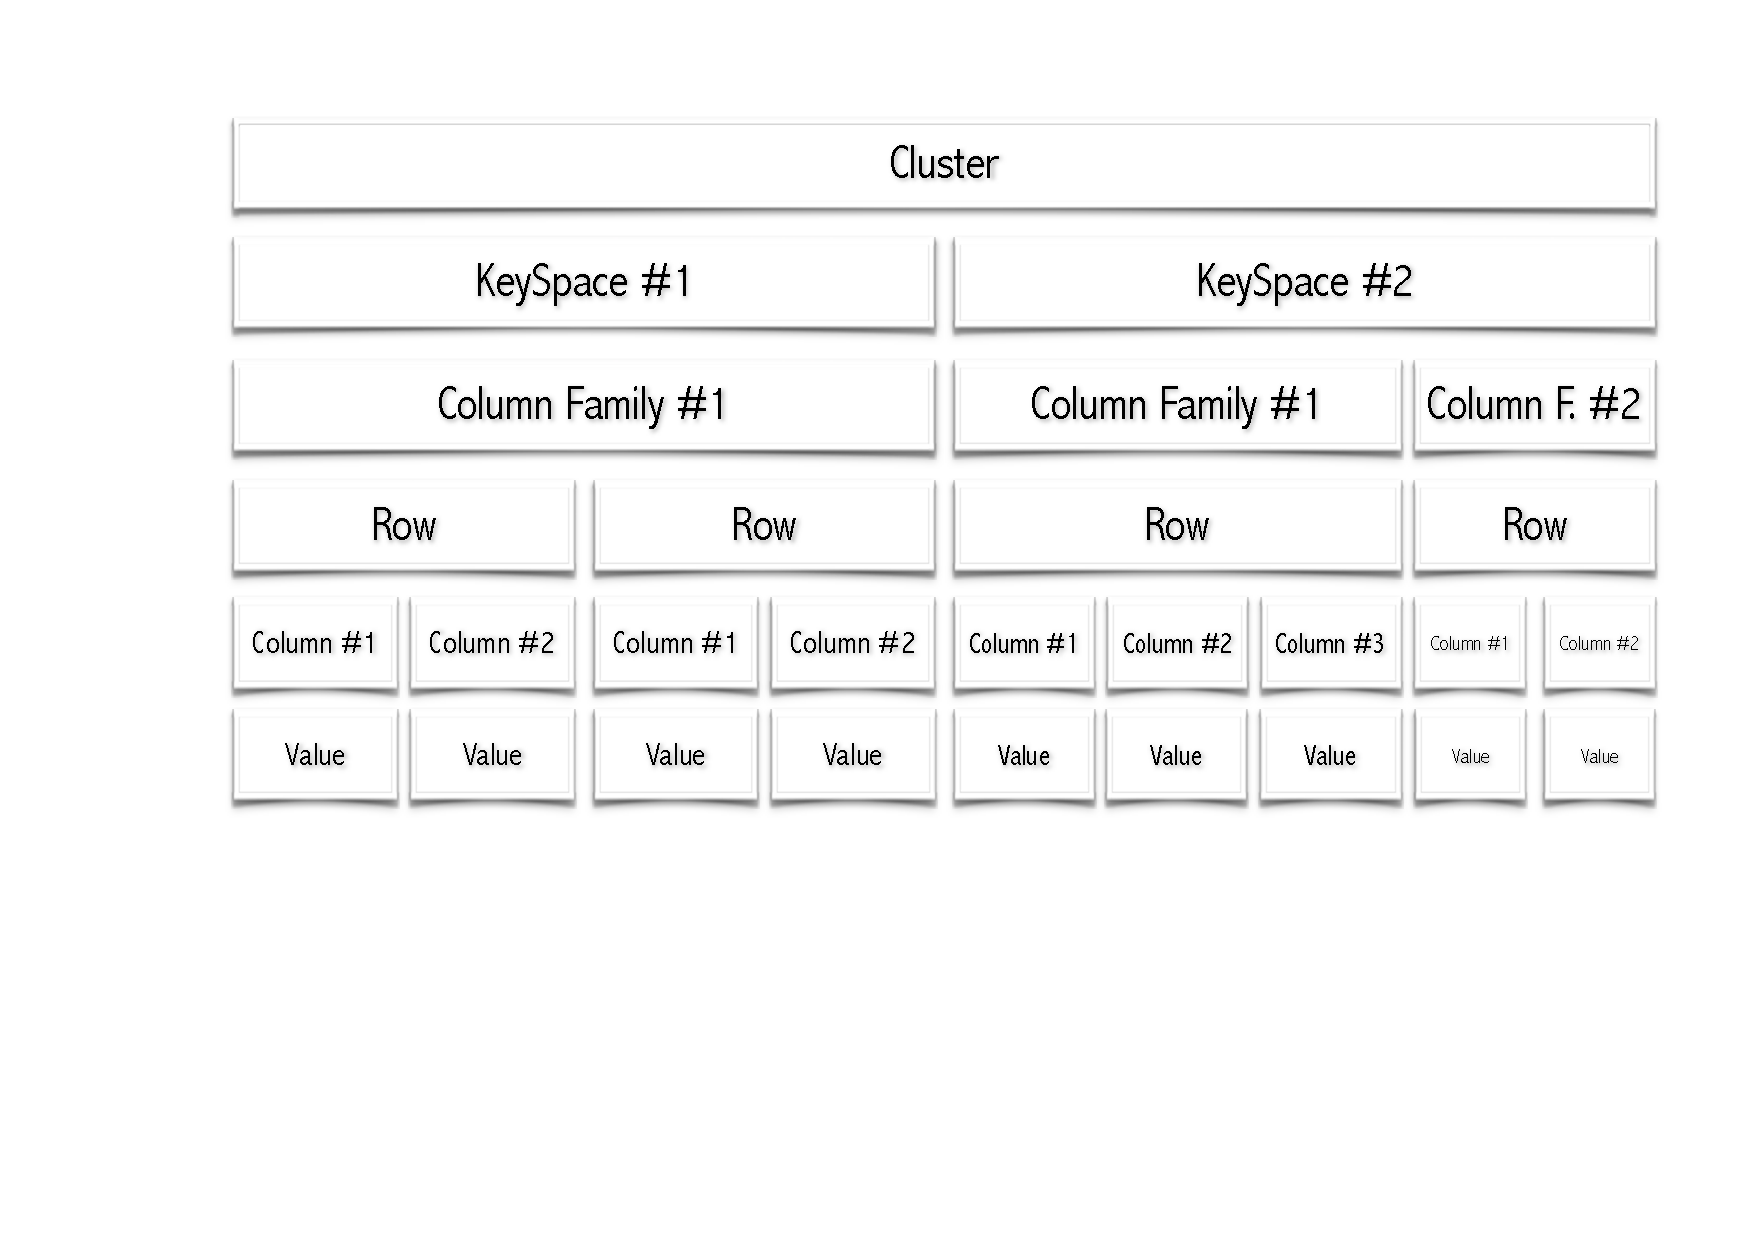
\includegraphics[trim = 25mm 70mm 15mm 15mm, clip, width=0.9\textwidth]{resources/cassandra/cassandraDataModel}
\caption[Datenmodell]{Datenmodell}
\label{img:cassandraDataModel}
\end{figure}
\cass\ definiert einen Datenbankserver als ein Cluster, auf dem mehrere Datenbanken (Keyspaces) angelegt werden. Eine Spaltenfamilie (Column Family) entspricht einer Tabelle und enthält Zeilen (Rows), welche mit einer eindeutigen Id zu identifizieren sind. In Zeilen (Rows) werden die Datensätze gespeichert, wobei jede Zeile bis zu 2 Milliarden Spalten (Columns) enthalten kann. Die Spalten (Columns) dagegen enthalten jeweils ein Paar „Schlüssel-Wert“ (Key-Value-Paar). 
Um bei Leseoperationen einen effizienteren Zugriff erreichen zu können, müssen die Spalten (Columns) Super Columns definieren, indem mehrere Spalten zusammengesetzt werden.


\section{Logikschicht (Backend)}
\subsection{Rest Server}

\subsection{Spring MVC}


\section{Präsentationsschicht (Frontend)}
AngularJS 2


\section{Frameworks}





Alllgemeine Architektur
    Überblick
    Datenschicht
        Nosql

Frameworks